\documentclass[USenglish,onecolumn]{article}

\usepackage[utf8]{inputenc}
\usepackage[big]{dgruyter}
\usepackage{booktabs,graphicx,longtable}
\usepackage{algorithm}
\usepackage{algpseudocode}
\makeatletter\providecommand{\plist@algorithm}{}\makeatother
\usepackage{url}

\setcounter{secnumdepth}{2}
\begin{document}

\articletype{Research Article{\hfill}Open Access}

\author[1]{Quang-Vinh Dang}

\author*[2]{Dat Le}

\author[3]{Minh Ngoc Dinh}

\affil[1]{British University Vietnam, Hung Yen, Vietnam; E-mail: vinh.dq4@buv.edu.vn; ORCID: 0000-0002-3877-8024}

\affil[2]{Department of Science, Technology, and International Projects, Ho Chi Minh City University of Economics and Finance, Ho Chi Minh City, 700000, Vietnam; E-mail: datla@uef.edu.vn; ORCID: 0009-0005-5038-8570}

\affil[3]{Millennia Education, Ho Chi Minh City, Vietnam; E-mail: minh.dinh@maeducation.com; ORCID: 0000-0003-4026-6068}

\title{\huge What can real cause--effect benchmarks resolve? Sampling noise, marginal shortcuts and assumption regimes}

\runningtitle{What can real cause--effect benchmarks resolve?}

\begin{abstract}
{Causal-discovery methods are compared by small accuracy gains on a few real benchmarks. We ask what these benchmarks can resolve and why rules that test the conditional structure of a pair rarely beat simple rules. Twelve direction rules were run under one protocol fixed before the runs on eight real pair collections (four new) and on graph benchmarks. No rule leads across collections. On $102$ T\"ubingen pairs a paired test needs a difference of $19$ accuracy points for $80\%$ power, and among ten non-degenerate rules no pairwise difference reaches a raw $p<0.05$. Unreported conventions move a rule as much: a rounding convention that a baseline's description does not fix changes its weighted accuracy by six points, and the treatment of tied values changes IGCI from $94\%$ to $6\%$ on one collection. Two mechanisms are supported: the chamber pairs can be oriented from the marginals alone, a property of their actuator-to-sensor design, and additive-noise rules are near-perfect when the noise scale is independent of the cause and reversed when it depends on it. Attempts to turn this into a rule or a predictive model fail their predictions fixed in advance, so the account is partial. We give recommendations.}
\end{abstract}
\keywords{causal discovery, cause--effect pairs, benchmark evaluation, reproducibility, additive noise models}
\classification[MSC]{62D20, 68T05}

\journalname{Journal of Causal Inference}
\DOI{DOI}
\startpage{1}
\received{..}
\revised{..}
\accepted{..}
\journalyear{2026}
\journalvolume{1}

\maketitle

\section{Introduction}\label{sec:intro}

Cause--effect benchmarks drive method development in causal discovery. For two variables the reference is the T\"ubingen collection \citep{mooij2016distinguishing}, 108 pairs of real measurements of which 102 are univariate; for graphs it is the protein-signalling data of \citet{sachs2005causal} with 17 consensus arcs. A new rule is typically presented in a table in which its number is larger than those of earlier rules. This paper asks how much information such a table carries. It runs a panel of direction rules under one protocol fixed before the runs on eight real pair collections, and asks how large a difference the benchmarks can resolve and why rules that test the conditional structure of a pair \citep{hoyer2009nonlinear,peters2014identifiability,hyvarinen2013pairwise,immer2023loci,lorch2022amortized} so rarely beat simpler rules that read the scale of regression errors or the marginal density \citep{blobaum2018cause,daniusis2010inferring,stienstra2026oneruler}. On T\"ubingen all of them lie between $55\%$ and $67\%$ with intervals of $\pm10$ points; the ordering of the rules on the Causal Chambers \citep{gamella2025chamber} is negatively, but not significantly, correlated with it.

\paragraph{Contributions.} (1) A same-protocol comparison of twelve pair rules on eight real collections (T\"ubingen; six Causal Chambers collections, four of them new; the Sachs pairs), with the stored decision of every rule on every pair, cluster-aware inference and a reproduction of a published headline number (Section~\ref{sec:conventions}). (2) A resolution analysis: a paired test on $102$ pairs has $80\%$ power only for a difference of about $19$ accuracy points, and among ten non-degenerate rules none of $45$ comparisons reaches a raw $p<0.05$; ten reporting universes move a single rule by $11$ to $26$ points and its rank by up to nine places, and $50$ preprocessing configurations by $7$ to $22$ points (Section~\ref{sec:results}). (3) Two unreported implementation conventions, the rounding of a quantiser and the treatment of tied values, that move a rule's accuracy by six and by up to $88$ points (Section~\ref{sec:conventions}). (4) Mechanism evidence, tested by prediction, matched manipulation with a control and leakage-free validation (Section~\ref{sec:mech}): the chamber collections, whose causes are experimenter-set actuators, can be oriented from their marginals alone, a cue that does not transfer to T\"ubingen; additive-noise rules are near-perfect when the noise scale does not depend on the cause and reversed when it does; two attempts to build a rule or a predictive model on this account fail their predictions fixed in advance, which bounds it. (5) Recommendations for reporting (Section~\ref{sec:discussion}), and an accounting of the attempts to build a better rule (Appendix~\ref{app:negative}).

\subsection{Related work}\label{sec:related}
\emph{Direction rules.} Identifiability results for linear non-Gaussian \citep{shimizu2006linear}, additive-noise \citep{hoyer2009nonlinear,peters2014identifiability,zhang2009identifiability} and post-nonlinear models underlie most pair rules; IGCI \citep{daniusis2010inferring} rests on the independence of the cause distribution and the mechanism, RECI \citep{blobaum2018cause} compares regression errors after scaling, LOCI \citep{immer2023loci} fits location-scale models, SLOPE \citep{marx2017slope} uses minimum description length, and learned rules are trained on simulated pairs \citep{lopezpaz2015towards,lorch2022amortized}. \emph{Evaluation.} Real data with known cause--effect structure are scarce: T\"ubingen for pairs, the Causal Chambers \citep{gamella2025chamber} for physical devices with a documented graph, and the Sachs network, a consensus rather than a ground truth. On simulated graphs, \citet{reisach2021beware} showed that the variance structure of additive-noise models can be read by a trivial rule; our marginal-only classifier is a pair-level analogue on real data. A same-hands re-evaluation on T\"ubingen that also introduced the compression baseline we use is \citet{stienstra2026oneruler}; we reproduce its main figure. For graphs we also ran BF-BIC with BOSS \citep{ramsey2025bfbic} and an SNOE-style \citep{huang2025snoe} orientation (Appendix~\ref{sec:graphs}).

\emph{What this paper does not claim.} It does not claim that published methods misreport their results; we audited one published table and reproduced it. It does not claim that dependence-based methods are worse in general: they are among the best rules in the regimes that fit their assumptions and the worst in others, and a benchmark that mixes regimes averages them.

\section{Collections, rules and protocol}\label{sec:data}

\subsection{Pair collections}\label{sec:collections}
Table~\ref{tab:collections} lists the eight collections (the seventh, the walks of all $19$ untouched recordings, contains the five recordings of the walk collection and fourteen more). A \emph{pair} is an ordered pair of variables with a known direction; the cause is the first variable of an edge of the documented graph. Two features of the table matter for every later statement. First, only T\"ubingen is a collection of unrelated mechanisms; the six others consist of pairs taken from one or two devices, so the number of \emph{distinct edges} is much smaller than the number of pair-runs (47 distinct edges behind the 94 i.i.d.\ chamber pair-runs, at most 65 distinct cause--effect names behind the 122 walk pairs, 8 behind the Bernoulli collection, 7 behind the changepoint collection and 4 behind the Malus collection, whose pairs share their cause variable). Intervals and tests that treat pairs as independent therefore overstate the information; Appendix Table~\ref{tab:collections_ci} gives cluster-bootstrap intervals (clusters: distinct edge, or recording for the walks). Second, in the chamber collections the cause is an actuator whose value the experimenter sets, which gives it a recognisable marginal law (uniform on a grid of levels, piecewise constant, a random walk) while the effects are sensors.

\begin{table}[t]
\caption{The eight real pair collections. ``Pairs'': pair-runs scored; ``edges'': distinct edges of the documented graph; ``units'': independent recordings or experiments. Rows: rows per pair after the cap of $2000$ random rows (T\"ubingen: at most $2000$ rows, dequantised; chamber collections: raw values).}
\label{tab:collections}
\small
\begin{tabular}{@{}lccccp{5.6cm}@{}}
\toprule
Collection & Pairs & Edges & Units & Rows & Source and cause\\
\midrule
T\"ubingen & 102 & 102 & 102 & $\le 2000$ & Univariate pairs of the CEP benchmark \citep{mooij2016distinguishing}; official weights\\
Chambers iid & 94 & 47 & 2 & 2000 & Wind and light tunnel with i.i.d.\ actuator settings \citep{gamella2025chamber}; two seeds per edge\\
Walks, all 19 & 486 & $\le65$ & 19 & 2000 & All untouched recordings (wind-tunnel random-walk actuators, the pressure-control recording, light-tunnel walks); every edge of each documented graph\\
Chambers walks & 122 & $\le65$ & 5 & 2000 & First recording of each type of random-walk experiments (actuators are random walks); the same cause--effect names recur across the five recordings\\
Sachs & 17 & 17 & 1 & 853 & Consensus arcs among 11 proteins, log scale \citep{sachs2005causal}\\
Bernoulli & 16 & 8 & 1 & 2000 & Wind tunnel, \texttt{random\_loads\_both}; the cause \texttt{load\_in} takes $101$ levels (steps of $0.01$), so after subsampling it has about $20$ rows per value; cause always \texttt{load\_in}\\
Changepoints & 70 & 7 & 10 & 2000 & Wind tunnel, piecewise-constant actuator (change points); cause always \texttt{load\_in}\\
Malus & 48 & 4 & 12 & 1000 & Light tunnel with polarisers, Malus's law; causes \texttt{pol\_1}, \texttt{pol\_2}\\
\bottomrule
\end{tabular}
\end{table}

Table~\ref{tab:diag} describes the collections with the quantities used later: the median number of rows, the median absolute Spearman correlation, the median residual heteroscedasticity $h$ of Section~\ref{sec:regimes} (true direction), the median excess kurtosis of the cause and of the effect, the median number of distinct values of the cause, and the share of pairs with many ties (fewer distinct values than $90\%$ of the rows) in either variable before any jitter (T\"ubingen is reported after dequantisation, hence zero). Figure~\ref{fig:examples} shows one randomly chosen pair per collection.

\begin{table}[t]
\caption{Descriptive diagnostics of the seven original collections (medians over pairs unless stated; the $486$-pair walk collection has the same kind of pairs as the walk collection).}
\label{tab:diag}
\small
\begin{tabular}{@{}lcccccccc@{}}
\toprule
Collection & Pairs & $n$ & $|\rho_S|$ & $h$ & kurt. cause & kurt. effect & distinct cause values & ties\\
\midrule
T\"ubingen & 102 & 392 & 0.50 & 0.18 & -0.2 & 0.2 & 392 & 0.00\\
Chambers iid & 94 & 2000 & 0.27 & 0.02 & -1.2 & -0.4 & 86 & 1.00\\
Chambers walks & 122 & 2000 & 0.26 & 0.08 & -1.2 & -0.6 & 255 & 1.00\\
Sachs & 17 & 853 & 0.08 & 0.08 & 3.1 & 2.3 & 276 & 1.00\\
Bernoulli & 16 & 2000 & 0.53 & 0.18 & -1.2 & -1.2 & 101 & 1.00\\
Changepoints & 70 & 1983 & 0.45 & 0.22 & -0.7 & -0.1 & 4 & 1.00\\
Malus & 48 & 1000 & 0.02 & 0.02 & -1.2 & -1.4 & 732 & 1.00\\
\bottomrule
\end{tabular}
\end{table}

\begin{figure}[t]
\centering
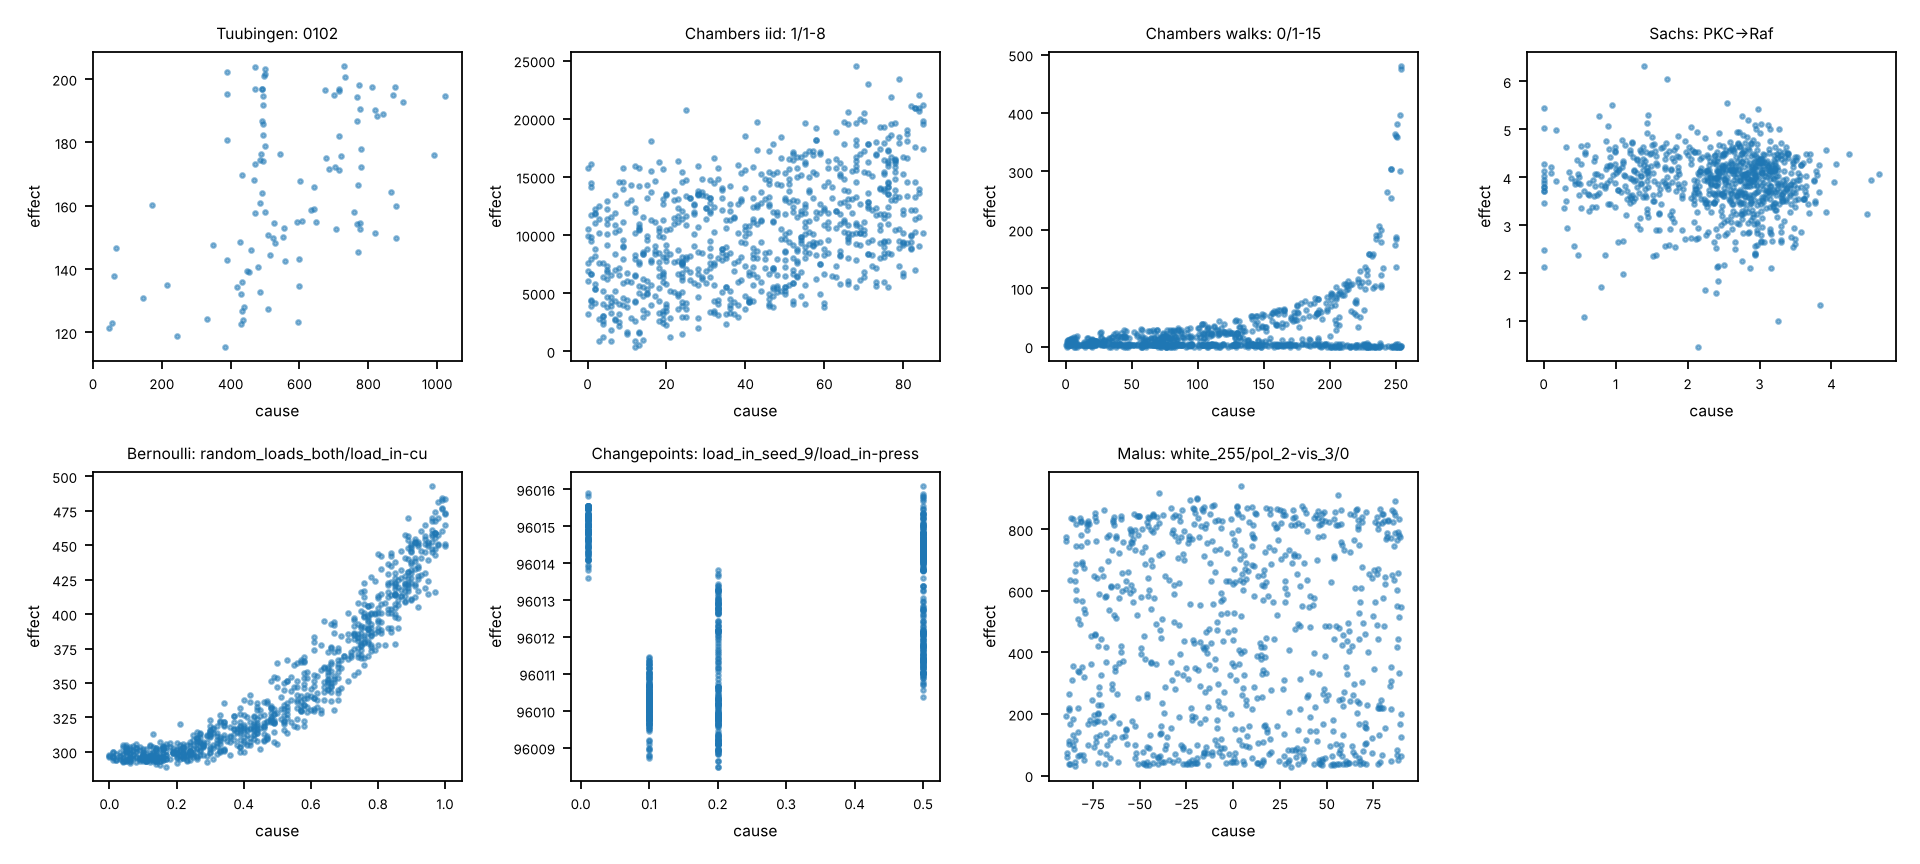
\includegraphics[width=\linewidth]{figs/examples.png}
\caption{One randomly chosen pair (seed $7$) from each collection; $800$ random rows, cause on the horizontal axis.}
\label{fig:examples}
\end{figure}

\subsection{Rules}\label{sec:rules}
Twelve rules, all run by us. Each returns a score whose sign gives the direction; a score of exactly zero counts as half correct. Settings were fixed in the script before the run (Appendix~\ref{app:prereg}) and none was tuned on a collection in which it is scored. \emph{Tie handling:} every rule receives the raw arrays (ties kept), as for the chambers in the first experiments; T\"ubingen arrays are dequantised (experiment 14) and have no ties. Giving the rules a copy with a $10^{-6}$ jitter on tied values reverses IGCI (Section~\ref{sec:ties}) and breaks TRA's spline fit, so jitter is used only in the sensitivity analysis of Section~\ref{sec:ties} and for the simulations.
\begin{itemize}
\item \textbf{IGCI} \citep{daniusis2010inferring}: entropy estimator with a uniform reference. \textbf{RECI} \citep{blobaum2018cause}: the direction with the smaller regression error of a spline fit after min--max scaling. Both are short re-implementations (\texttt{sprint\_cd/\allowbreak pair\_baselines.py}).
\item \textbf{ANM-HSIC} \citep{hoyer2009nonlinear}: additive-noise model with a spline regression and an HSIC independence test; \textbf{ANM-GP}: the \texttt{causal-learn} Gaussian-process version on $400$ rows; \textbf{RESIT} (\texttt{lingam}): random-forest regression of depth $4$ with $\alpha=0.01$.
\item \textbf{Pairwise LiNGAM} \citep{hyvarinen2013pairwise}: first-order likelihood-ratio statistic.
\item \textbf{LOCI} \citep{immer2023loci}: the authors' code in its default setting (neural networks, $5000$ steps, HSIC test, at most $1000$ rows).
\item \textbf{Compression} \citep{stienstra2026oneruler}: quantise both variables to $256$ levels, sort one by the other (stable), take the first difference as \texttt{int8}, compress with bzip2 (level 9), and compare the two normalised lengths. Two variants: our first implementation (\texttt{floor}$(256q)$, rows capped at $2000$) and the \emph{faithful} variant that reproduces the published figure (\texttt{round}$(255q)$, all rows thinned linearly above $8000$, raw values; Section~\ref{sec:audit}).
\item \textbf{TRA} \citep{elbouchattaoui2026tra}: cross-fitted smoothing-spline residuals, a rank-uniform residual cloud and the zero-dimensional persistence of its minimum spanning tree in a window; the constants $\kappa=1$, $c_\beta=4$, five folds, at most $1000$ rows are ours because the preprint does not fix them. It returns no value when the spline fit is ill-posed (cause with many tied values), which excludes it from the collections with binary or piecewise-constant causes.
\item \textbf{AVICI} \citep{lorch2022amortized}: the pretrained \texttt{scm-v0} model on the two-variable input, score $P(x\to y)-P(y\to x)$ (run in a separate environment with pinned JAX).
\item \textbf{PDM}: a gradient-boosting classifier trained on simulated pairs with $32$ features (ours; Appendix~\ref{app:negative}).
\end{itemize}
Reference implementations of IGCI, RECI, CDS, ANM and BivariateFit from the \texttt{cdt} package (v0.6.0, defaults) were also run to check ours (experiment 55; Section~\ref{sec:ties}). Not run: PNL (880\,s per pair on $400$ rows), CAM and SCORE (no package available offline), SLOPE (code not run), and rules that need the authors' trained weights.

\subsection{Protocol and provenance}\label{sec:protocol}
Every evaluation script was committed before it was run; Appendix~\ref{app:prereg} lists the 46 experiment scripts (numbers 17 to 60; 31 and 34 have two parts) with the commit that fixed them. Stored per-pair decisions are in \texttt{results/}, and every number in this paper is computed from them by the scripts in \texttt{scripts/}. Three analyses were designed after seeing per-pair results and are labelled as such where they appear: the multiverse and subset analyses of Sections~\ref{sec:multi}--\ref{sec:subsets}, the terciles of Table~\ref{tab:strata}, and the revised protocol of Section~\ref{sec:predict}. The study includes departures that we report rather than hide: our first compression implementation was wrong in a detail that the published text does not fix; the first run of the marginal-only classifier leaked information between training and test variables; one pre-registered test (Section~\ref{sec:predict}) was invalid as implemented and was rerun in a revised form, with both runs reported.

\section{Resolution, rankings and reporting freedom}\label{sec:results}

\subsection{No rule leads across collections}\label{sec:coll}

Appendix Table~\ref{tab:collections2} gives the accuracy of every rule on every collection (Figure~\ref{fig:collections} in the appendix).



\begin{figure}[t]
\centering
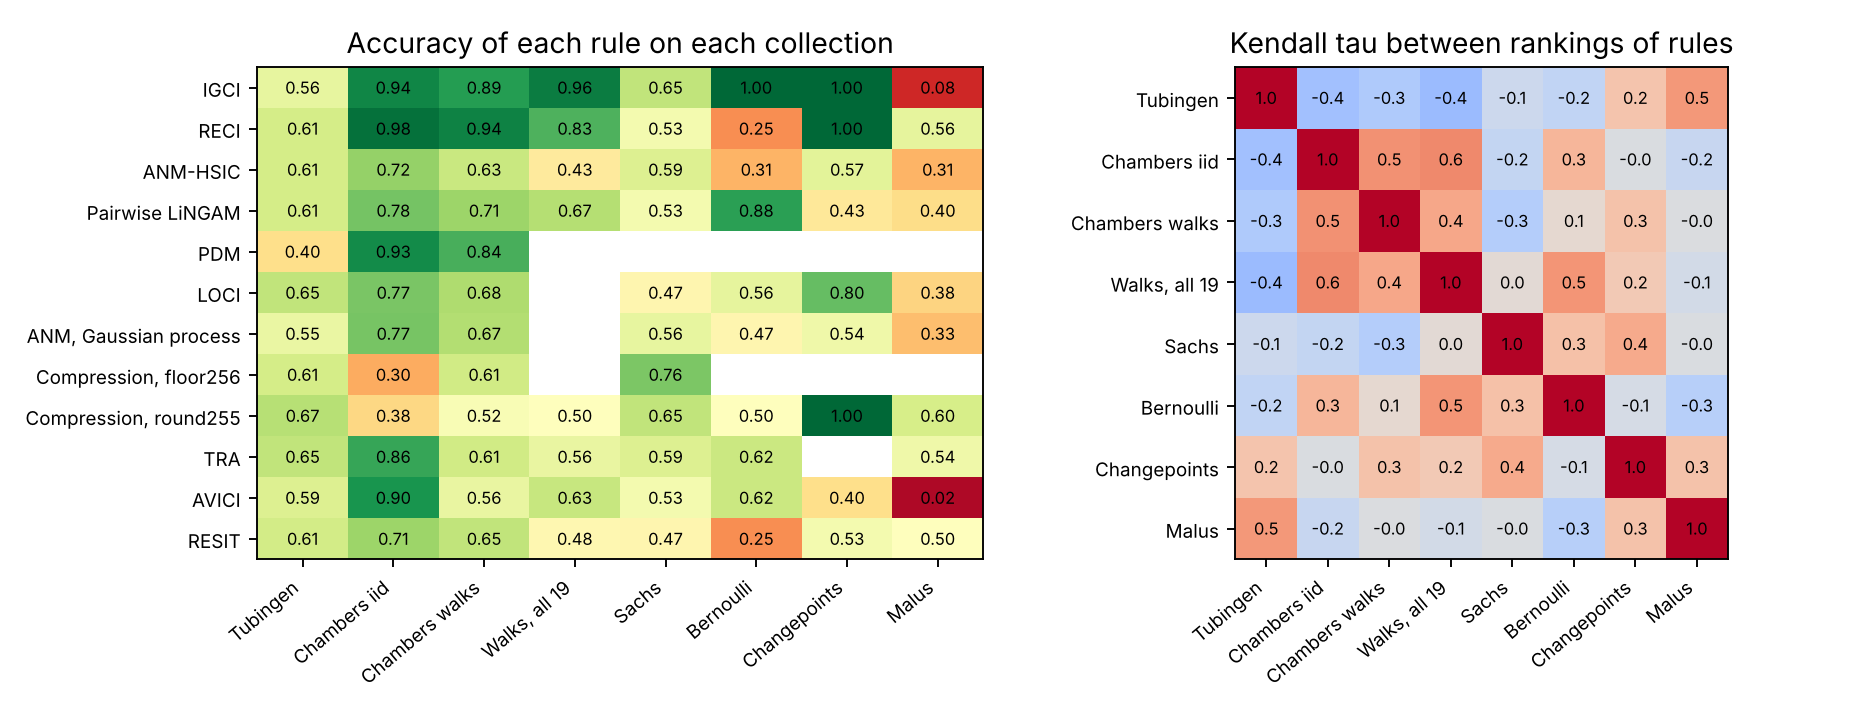
\includegraphics[width=\linewidth]{figs/collections.png}
\caption{Left: accuracy of every rule on every collection (all rules on raw arrays; T\"ubingen dequantised). Right: Kendall rank correlation between the orderings of the rules on two collections (rules run on both; at least five); none is distinguishable from zero after correction.}
\label{fig:collections}
\end{figure}

\paragraph{(1) The leader changes.} Round255 compression leads T\"ubingen ($66.7\%$; LOCI and TRA at $64.7$ and $64.6\%$) and Malus ($60.4\%$), RECI the two chamber collections with independent or random-walk actuators ($97.9\%$ and $94.3\%$), IGCI the $19$ untouched walk recordings ($95.7\%$; RECI $82.9\%$) and the Bernoulli collection ($100\%$), floor256 compression the $17$ Sachs pairs ($76.5\%$; round255 $64.7\%$), and IGCI, RECI and round255 compression tie on the changepoint pairs ($100\%$). Four of the twelve rules lead at least one collection. IGCI is above $70\%$ on five collections and at $8.3\%$ on Malus and $55.9\%$ on T\"ubingen; RECI is above $70\%$ on four; pairwise LiNGAM on three; no other rule on more than two. The additive-noise rules lead nowhere: ANM-HSIC is at $43.4\%$ on the $19$ walk recordings, RESIT at $47.5\%$.

\paragraph{(2) Rules that agree on one collection disagree on the next.} In our implementation IGCI orients the Bernoulli and changepoint pairs correctly in every case and the Malus pairs wrongly in $44$ of $48$. RECI is at $25\%$ on the Bernoulli pairs. The pretrained AVICI model, run on two-variable inputs, is at $90.4\%$ on the i.i.d.\ chambers and $2.1\%$ on Malus. Round255 compression is at $100\%$ on the changepoint pairs, $60.4\%$ on Malus and $38.3\%$ on the i.i.d.\ chambers. With the recordings as clusters, sign-flip tests give IGCI above RECI on the $19$ walk recordings ($p=0.019$) and RECI above ANM-HSIC, AVICI and pairwise LiNGAM ($p<0.001$); on the i.i.d.\ chambers ($47$ edges as clusters) RECI is above ANM-HSIC ($p<0.001$) and IGCI above ANM-HSIC ($p=0.012$), while IGCI and RECI are not separated ($p=0.63$); with five recordings the smallest attainable $p$ is $0.0625$.

\paragraph{(3) Rankings do not clearly transfer.} Kendall's $\tau$ between the ordering of the rules on T\"ubingen and on the i.i.d.\ chambers is $-0.38$, on the walks $-0.30$ ($-0.42$ for all $19$ recordings), on Sachs $-0.12$, on Bernoulli $-0.19$; it is $+0.24$ against the changepoints and $+0.51$ against Malus. Of the $28$ correlations one has a raw permutation $p<0.05$ (i.i.d.\ against walks, $0.02$) and none survives a Holm correction (smallest adjusted $p=0.49$): the T\"ubingen accuracies span twelve points with intervals of $\pm0.10$, so the ordering of the rules on that collection is mostly noise, and the data support no statement of agreement or disagreement between collections at the level of rank correlations.

\paragraph{Cautions.} The i.i.d., walk, Bernoulli, changepoint and Malus collections are best read as case studies of regimes of two devices, not as samples of mechanisms: they have $47$, $\le65$, $8$, $7$ and $4$ distinct edges, the cause is an experimenter-set actuator and the effect a sensor. Cluster-bootstrap intervals (Appendix Table~\ref{tab:collections_ci}) are degenerate with fewer than nine clusters. The T\"ubingen arrays are dequantised, a convention that matters (on raw arrays IGCI is at $63.8\%$ on average over the configurations of Section~\ref{sec:protocol_multiverse} against $52.4\%$ dequantised). The leads of round255 compression on T\"ubingen and Malus rest on one pair over LOCI ($p=0.88$) and on three points with four clusters.


\subsection{Sampling noise}\label{sec:noise}

Appendix Table~\ref{tab:multi} gives the accuracies on T\"ubingen with exact Clopper--Pearson intervals. The half-width is about $0.10$ for every rule, and the intervals treat the pairs as independent, which they are not exactly (the official weights downweight groups of similar pairs; unweighted accuracy is used). All rules are evaluated on the same pairs, so the right comparison between two rules is the exact McNemar test on the pairs on which exactly one is correct; exact ties (a score of zero) and pairs on which a rule returned no value (TRA, $20$ pairs) are left out of the discordant counts, so TRA is compared on a different sample.

\begin{figure}[t]
\centering
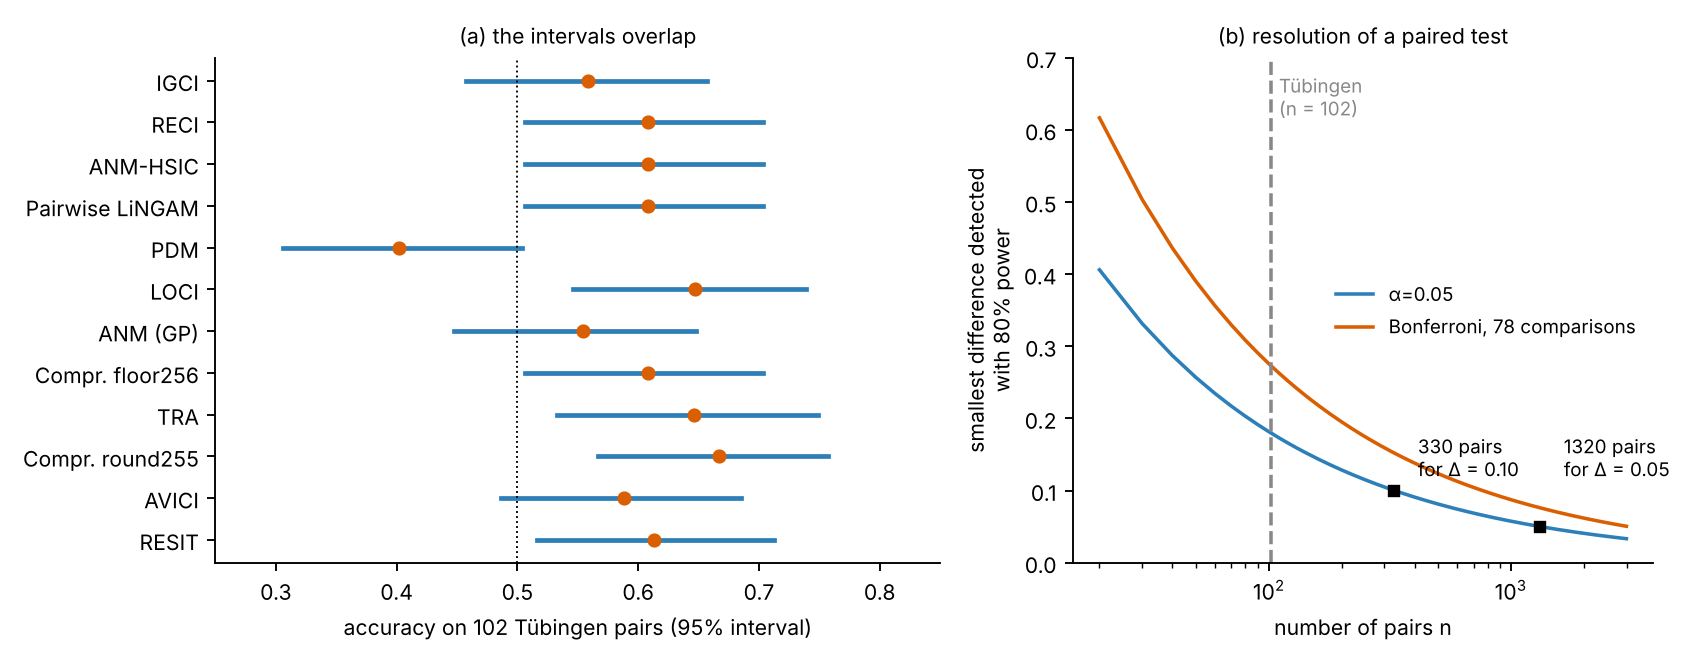
\includegraphics[width=\linewidth]{figs/fig3_resolution.png}
\caption{(a) Accuracy of the twelve rules on the $102$ T\"ubingen pairs with exact $95\%$ intervals. (b) Analytic smallest difference in accuracy detected with $80\%$ power by a paired test, as a function of the number of pairs, for a discordance rate of $0.42$.}
\label{fig:resolution}
\end{figure}

\paragraph{Two families of comparisons.} The first family has the twelve rules of Appendix Table~\ref{tab:collections2} plus the floor256 compression with raw rows: $78$ comparisons. Twelve have a raw $p<0.05$ and two survive a Holm correction (smallest adjusted $p=0.015$); both involve the learned classifier PDM, which is below chance (PDM against round255 compression and against LOCI; all $12$ raw-significant comparisons involve PDM), so they say nothing about the other rules. The second family fixes the ten rules that are not degenerate and not duplicated (IGCI, RECI, ANM-HSIC, pairwise LiNGAM, LOCI, ANM-GP, round255 compression, TRA, AVICI, RESIT; without PDM and without the other compression variants): $45$ comparisons, \emph{none} with a raw $p<0.05$ (smallest raw $p=0.11$, ANM-GP against RESIT). The result is the same on the common set of the $82$ pairs on which all ten rules return a value (exact ties counted as half in both cells of the discordance table): none of the $45$ comparisons has a raw $p<0.05$ (smallest $0.078$, ANM-GP against TRA). PDM's accuracy of $40.2\%$ is not a sign error: the same classifier and sign convention give $93\%$ and $84\%$ on the two chamber collections, so its failure on T\"ubingen is a failure to transfer from the simulator, which we did not diagnose further. For the best rule, round255 compression ($66.7\%$), the tests against RECI, LOCI, IGCI, ANM-GP and AVICI have $p=0.39$, $0.88$, $0.14$, $0.20$ and $0.35$ (discordant pairs $20$/$14$, $23$/$21$, $29$/$18$, $24$/$15$, $32$/$24$).

\paragraph{Detectable difference.} With the observed rate of discordant pairs ($42\%$, computed on pairs where both rules have a value and neither ties; averaged over the $78$ comparisons), a simulated paired comparison on $102$ pairs reaches $80\%$ power for a difference in accuracy of $0.19$ at level $0.05$ and of $0.27$ with a Bonferroni correction over the $78$ comparisons. The simulation draws the number of discordant pairs from the observed rate, splits them with the alternative probability, uses $1000$ replications per step of $0.01$, and treats pairs as independent. The figure agrees with the normal approximation of the exact test: with $n$ pairs and a fraction $d$ of discordant pairs, a difference in accuracy $\Delta$ is detected with power $1-\beta$ at level $\alpha$ when $\Delta\ge (z_{1-\alpha/2}+z_{1-\beta})\sqrt{d/n}$, which gives $0.180$ at $\alpha=0.05$ and $0.273$ at $\alpha=0.05/78$ for $n=102$, $d=0.42$. Inverting, the number of pairs needed to resolve a difference $\Delta$ at $80\%$ power is $7.85\,d/\Delta^2$: about $330$ pairs for $\Delta=0.10$, $1320$ for $0.05$ and $8240$ for $0.02$ at $d=0.42$. Differences of two to five points, which separate most of the rules in recent papers, are far below it: the collection cannot resolve them, whatever the rules.



\subsection{A multiverse of reporting choices}\label{sec:multi}

A reader of a pair-rule paper meets choices that are each reasonable and that each change the number: whether to use the benchmark's official weights; whether to restrict to pairs with enough rows; whether to report accuracy on all pairs or only on the pairs on which the rule is most confident (decided-only accuracy, as for a rule that abstains). We cross them: official weights or none; all pairs or only pairs with at least $250$, $500$ or $1000$ rows; accuracy on the $100$, $75$, $50$ or $25\%$ of the pairs with the largest absolute score. This gives $32$ universes. The coverage is taken exactly (top $k$ by $|\mathrm{score}|$, ties broken at random with a fixed seed); the score of several rules is not a calibrated confidence, so this is the operation a reader could apply, not each rule's own abstention. A universe is kept only if every rule is evaluated on at least $30$ pairs: $10$ of $32$ qualify (all pairs, or pairs with $\ge 250$ rows; coverage $100$, $75$, and for all pairs $50\%$; each with and without weights). The other $22$ (for example the $25\%$ of the $36$ pairs with at least $1000$ rows, which is nine pairs) cannot be reported. A first run kept them, and the ranges were far wider ($0.27$ to $0.75$ for IGCI, up to $1.00$ for RECI); an accuracy on nine pairs is not a defensible report, and we dropped them on review.

\paragraph{Results.} In the ten universes the accuracy of a single rule still moves by $11$ to $26$ points (Appendix Table~\ref{tab:multi}): $0.47$ to $0.71$ for IGCI, $0.61$ to $0.87$ for RECI, $0.67$ to $0.88$ for the round255 compression, $0.63$ to $0.77$ for LOCI. Ranks move by up to nine places (ANM-HSIC from third to twelfth, pairwise LiNGAM from fourth to thirteenth, RESIT from fifth to thirteenth); RESIT's score takes only the values $-1$, $0$, $1$, so its coverage ranking is mostly random tie-breaking and its range is not informative. Three rules are first in at least one universe: round255 compression in $8$, RECI and LOCI in $1$ each; the round255 compression is above RECI in $9$ universes and no other rule is above RECI in more than four. The coverage tie-breaking is immaterial except for RESIT: over $50$ tie-break seeds the range of every other rule is unchanged and the first counts are identical ($8$, $1$, $1$), while RESIT's range varies by $0.03$ (its score has only three values). Without the round255 variant in the panel RECI is first in $6$ universes, LOCI and TRA in $2$ and the raw-row floor256 compression in $1$. The first counts are over universes, not within one universe, ties share the first rank, and they depend on which variants of a rule are in the panel: the round255 compression convention was selected because it reproduces a published figure (Section~\ref{sec:audit}), and under the other conventions its unweighted accuracy ranges from $60.8\%$ to $69.6\%$, so its lead in $8$ of the $10$ universes is partly a consequence of that selection. TRA returned no value on $20$ pairs; these are excluded from its accuracy ($82$ pairs) and from its coverage ranking.

\begin{figure}[t]
\centering
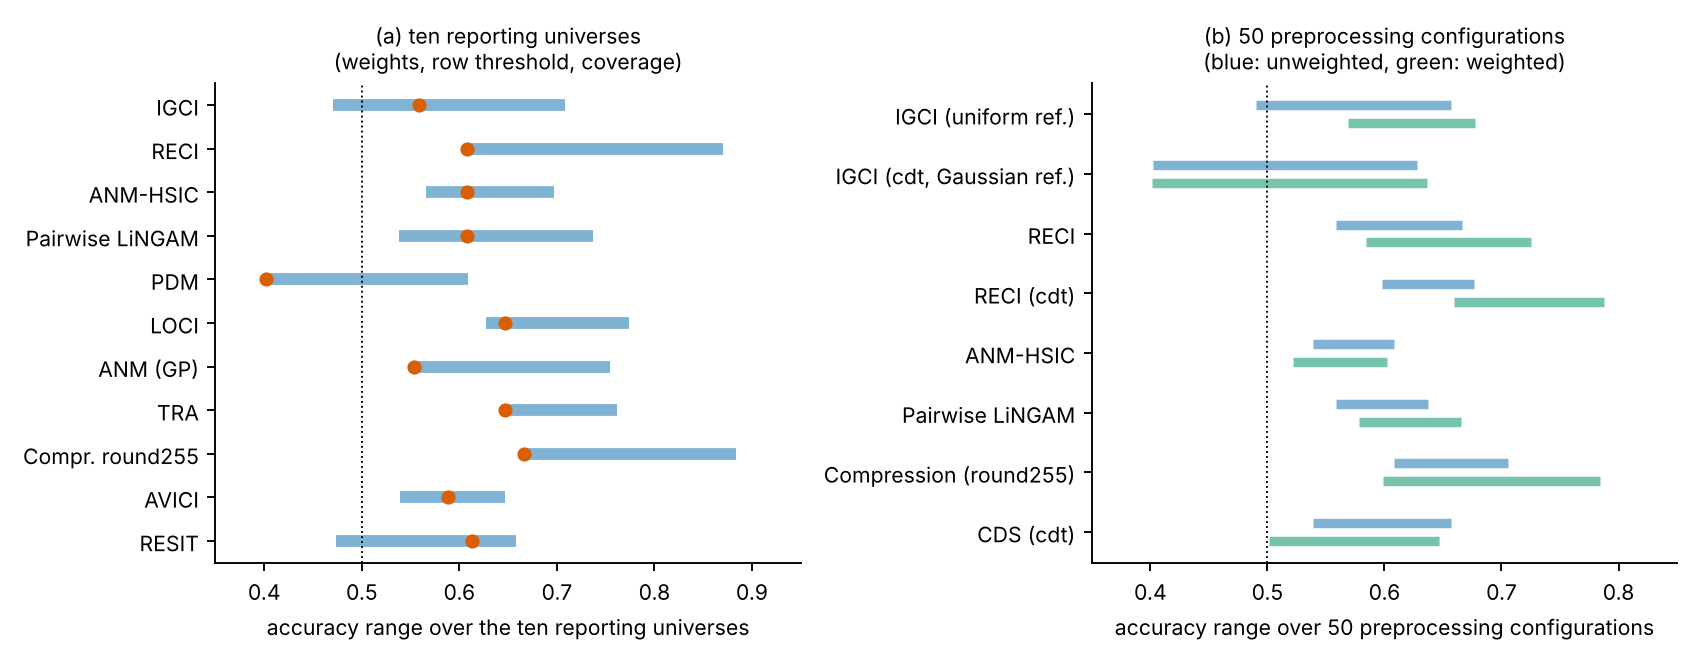
\includegraphics[width=\linewidth]{figs/fig4_freedom.png}
\caption{The range of each rule's accuracy on T\"ubingen (a) over ten defensible reporting universes (dot: accuracy on all pairs, unweighted) and (b) over $50$ preprocessing configurations (number of rows, dequantisation, seed).}
\label{fig:freedom}
\end{figure}

Single choices can be large. The official weights move RECI from $60.8\%$ to $70.9\%$, round255 compression from $66.7\%$ to $74.7\%$, and the floor256 variant from $60.8\%$ to $68.0\%$, while LOCI goes from $64.7\%$ to $63.9\%$. The quantisation convention of the compression rule (Section~\ref{sec:audit}) moves the weighted accuracy between $68.8$ and $74.7\%$.

Selecting among random subsets of $50$ pairs inflates the expected best accuracy of every rule by seven to eight points after ten tries without changing the order of the rules (Appendix~\ref{app:subsets}).

\subsection{A protocol multiverse on T\"ubingen}\label{sec:protocol_multiverse}

Section~\ref{sec:multi} varied how a result is reported. Here we vary how the data are prepared, for the same rule and the same pairs (experiment 61): the number of rows ($250$, $500$, $1000$, $2000$ or all, drawn at random), whether tied values are dequantised, and the seed (which changes the subsample and the rule's own randomness): $50$ configurations. Appendix Table~\ref{tab:protocol} gives the range of each rule's accuracy and the range of the marginal means of each factor.



The same rule on the same pairs moves by $7$ to $22$ points unweighted and $8$ to $23$ points weighted: IGCI with a uniform reference from $49.0$ to $65.7\%$, with cdt's Gaussian reference from $40.2$ to $62.7\%$ (the dequantisation alone: $52.4\%$ against $63.8\%$ on average for ours, so on raw T\"ubingen arrays IGCI is better than RECI, and with dequantisation worse), RECI weighted from $58.4$ to $72.5\%$, round255 compression weighted from $59.9$ to $78.4\%$, CDS unweighted from $53.9$ to $65.7\%$. The number of rows matters little on average (a few points) but through the random subsample the seed alone moves RECI, LiNGAM and ANM-HSIC by two to three points. The range of a single rule across protocol choices is as large as the range between the twelve rules of Appendix Table~\ref{tab:collections2} on T\"ubingen ($40$ to $67\%$, or $55$ to $67\%$ without the classifier below chance), and larger than the $2$ to $5$ points by which methods are usually separated. A comparison between two rules is therefore informative only under one identical protocol, run with the same preprocessing and several seeds; a comparison against a number quoted from a paper is not.

\section{Implementation conventions: reproduction audit and tie handling}\label{sec:conventions}

\subsection{A reproduction audit}\label{sec:audit}

We audited one published table in detail, because it is the one for which the protocol is specified closely enough to repeat and for which the claims concern exactly the question of this paper. \citet{stienstra2026oneruler} re-evaluate bivariate rules on the same $102$ T\"ubingen pairs with the official weights, no tuning and a decision forced on every pair. They report $74.7\%$ weighted accuracy for a parameter-free compression rule ($68$ of $102$ pairs, $66.7\%$ unweighted), $76.0\%$ for the same rule on the $100$ pairs on which SLOPE \citep{marx2017slope} is evaluated, $77.2\%$ for SLOPE under a forced decision on those pairs (from the authors' stored output) and $82.4\%$ as published (a decided-subset figure; $81.7\%$ when the pairs answered by SLOPE's significance test are scored), and $70.7\%$ for a faithful re-run of RECI; they trace the commonly quoted $77.5\%$ for RECI to a mis-copied cell. Their point is that figures obtained with test-set model selection or with abstention gated by a significance test are not comparable with forced-decision figures.

\paragraph{What we reproduce.} Our RECI re-implementation gives $70.9\%$ weighted (and $60.8\%$ unweighted) on the same pairs, within $0.2$ points of their $70.7\%$. Compression is the instructive case (Table~\ref{tab:audit}). Our floor256 variant followed the published description (both variables quantised to $256$ levels by linear min--max scaling, stable sort, first difference as \texttt{int8}, bzip2 level 9, normalised lengths, sign of the difference) but with the quantiser $\lfloor 256\,q\rfloor$ clipped to $255$, and with the rows capped at $2000$ and dequantised in the variant we ran at first; it gave $60.8\%$ (dequantised) and $64.7\%$ (raw rows), and $68.0\%$ and $65.9\%$ weighted. The text does not state how the integer levels are obtained from the scaled values. With $\mathrm{round}(255\,q)$, all rows (linearly thinned above $8000$) and raw values the same code gives exactly $68$ of $102$ pairs and $74.66\%$ weighted: the published figure. With $\lfloor 255\,q\rfloor$ it gives $71$ pairs and $70.5\%$. A one-pair difference in the count moves the weighted accuracy by up to six points because the official weights are unequal. Capping the rows changes the round255 variant by at most four weighted points ($71.7\%$ at $500$ rows, $74.4\%$ at $2000$, $74.7\%$ at $8000$, $75.3\%$ without thinning) and the floor variant by up to eight ($62.7$ to $70.8\%$); the conventions and caps are in \texttt{results/exp54\_audit\_conventions.json}. We adopted the round255 convention only after the reproduction check against the published figure, from three quantisation conventions and six row caps (all $18$ in Appendix Table~\ref{tab:grid18}), and we say so: it is chosen to match a published target, not to maximise accuracy on any data of ours, and the exact match is fragile to the row cap.

\begin{table}[t]
\caption{Reproduction of the compression baseline on the $102$ T\"ubingen pairs (official weights). The published value is $68$ of $102$ pairs, $74.7\%$ weighted.}
\label{tab:audit}
\small
\begin{tabular}{@{}lccc@{}}
\toprule
Quantisation and rows & pairs correct & unweighted & weighted\\
\midrule
$\lfloor 256q\rfloor$, all rows & 67 & 0.657 & 0.688\\
$\lfloor 255q\rfloor$, all rows & 71 & 0.696 & 0.705\\
$\mathrm{round}(255q)$, all rows & 68 & 0.667 & 0.747\\
$\mathrm{round}(255q)$, $2000$ rows & 69 & 0.676 & 0.744\\
$\mathrm{round}(255q)$, no thinning & 69 & 0.676 & 0.753\\
$\mathrm{round}(255q)$, $500$ rows & 71 & 0.696 & 0.717\\
floor256, $2000$ random dequantised rows (experiment 42) & 62 & 0.608 & 0.680\\
\bottomrule
\end{tabular}
\end{table}

\paragraph{What we do not reproduce or compare.} We did not run SLOPE, and so cannot confirm the $77.2\%$ or $82.4\%$ figures. For LOCI, our run of the authors' code gives $64.7\%$ unweighted and $63.9\%$ weighted ($65.7\%$ and $66.4\%$ with $2000$ rows instead of $1000$); we did not locate a published T\"ubingen accuracy for LOCI that we could verify offline and make no comparison. The TRA preprint does not fix the constants we had to choose; our $64.6\%$ on the $82$ pairs it scores is for our constants and is not a test of its claims. SNOE, BF-BIC and AVICI make claims on graphs or simulated data that we did not attempt to reproduce.

\paragraph{What the audit shows for the argument.} (i) Two numbers that a reader would call ``the compression baseline on T\"ubingen'' differ by six weighted points because of a rounding convention that the description does not fix (the quantiser $\lfloor 256q\rfloor$ against $\mathrm{round}(255q)$; rounding alone, $\lfloor 255q\rfloor$ against $\mathrm{round}(255q)$, is $4.2$ points); a comparison between methods whose gaps are three to five points is therefore inside the variation produced by conventions that the descriptions we checked do not fix. (ii) The reproduced baseline is, on T\"ubingen, among the best rules in our panel ($66.7\%$, $74.7\%$ weighted), above RECI and LOCI but not significantly (exact McNemar $p=0.39$ and $0.88$), and it is at $38.3\%$ on the i.i.d.\ chamber pairs, where RECI is at $97.9\%$. (iii) Its authors state that the rule's signal is partly marginal-geometric (a rank transform of the inputs, which flattens marginal shape, costs sixteen points in their experiments); this is the mechanism of Section~\ref{sec:marg}.

\subsection{Tie handling and implementation variants}\label{sec:ties}

The compression audit of Section~\ref{sec:audit} is one case of a general problem: choices that no paper reports and that a rule is sensitive to. Two more we measured.

\paragraph{Ties reverse IGCI.} The chamber arrays contain many tied values (discretised sensors, actuator levels). IGCI estimates the entropy of each scaled variable from the spacings between consecutive sorted values and prefers the direction in which the effect has the smaller entropy. Our implementation discards zero spacings; the alternative is to break ties with a tiny jitter, which turns the repeated values into spacings of order $10^{-6}$ and lowers the entropy of the tied variable. Table~\ref{tab:ties} gives the accuracy of IGCI under the two conditions on every collection (experiment 59, the same pairs): on the raw arrays $94\%$ on the i.i.d.\ chamber pairs, $89\%$ on the walk pairs, $100\%$ on the Bernoulli and the changepoint pairs and $8\%$ on Malus; with a jitter of one millionth of the range on the tied values $6\%$, $13\%$, $0\%$, $0\%$ and $94\%$. The two conditions give approximately complementary accuracies ($a$ against $1-a$) on the collections with many ties (i.i.d.\ chambers $0.94$ and $0.06$, Bernoulli and changepoints $1.00$ and $0.00$, Malus $0.08$ and $0.94$, walks $0.89$ and $0.13$), and not on Sachs ($0.65$ and $0.47$), so for most collections the verdict that IGCI is ``best on the chambers'' or ``best on Malus'' is determined by a convention of one line of code. T\"ubingen, which is dequantised in both conditions and so has no ties, is unaffected ($55.9\%$); on the raw T\"ubingen arrays, however, IGCI is at $63.8\%$ on average over the protocol configurations of Section~\ref{sec:protocol_multiverse} against $52.4\%$ when they are dequantised. RECI, pairwise LiNGAM and the cdt version of RECI do not change; cdt's CDS changes by up to six points (Sachs $0.53$ to $0.59$); ANM-HSIC changes by up to ten points on one collection (changepoints, $0.57$ raw, $0.47$ jittered). TRA fails on the jittered arrays (its smoothing-spline fit is ill-posed) and works on the raw ones. We use the raw arrays for every rule (Section~\ref{sec:rules}). A first pass of this study gave the new collections the jittered arrays, reported IGCI at $0\%$ on the Bernoulli and the changepoint pairs and offered a conjecture about it; the conjecture was wrong, the cause was the jitter, and the stored raw results replace that analysis.

\begin{table}[t]
\caption{Accuracy of rules under two tie conditions (raw arrays; $10^{-6}$ range jitter on tied values), same pairs (experiment 59). T\"ubingen is dequantised in both. cdt: \texttt{cdt} package defaults.}
\label{tab:ties}
\small
\setlength{\tabcolsep}{3pt}
\begin{tabular}{@{}llccccccc@{}}
\toprule
Rule & Ties & T\"ub. & iid & walks & Sachs & Bern. & Chgpt. & Malus\\
\midrule
IGCI (ours, uniform reference) & raw & 0.56 & 0.94 & 0.89 & 0.65 & 1.00 & 1.00 & 0.08\\
IGCI (ours, uniform reference) & jitter & 0.56 & 0.06 & 0.13 & 0.47 & 0.00 & 0.00 & 0.94\\
IGCI (cdt, Gaussian reference) & raw & 0.42 & 0.94 & 0.84 & 0.47 & 1.00 & 1.00 & 0.08\\
IGCI (cdt, Gaussian reference) & jitter & 0.42 & 0.06 & 0.12 & 0.53 & 0.00 & 0.00 & 0.94\\
ANM-HSIC & raw & 0.57 & 0.73 & 0.62 & 0.59 & 0.31 & 0.57 & 0.31\\
ANM-HSIC & jitter & 0.57 & 0.72 & 0.62 & 0.59 & 0.31 & 0.47 & 0.33\\
RECI & raw & 0.61 & 0.98 & 0.94 & 0.53 & 0.25 & 1.00 & 0.56\\
RECI & jitter & 0.61 & 0.98 & 0.94 & 0.53 & 0.25 & 1.00 & 0.56\\
Pairwise LiNGAM & raw & 0.61 & 0.78 & 0.71 & 0.53 & 0.88 & 0.43 & 0.40\\
Pairwise LiNGAM & jitter & 0.61 & 0.78 & 0.71 & 0.53 & 0.88 & 0.43 & 0.40\\
\bottomrule
\end{tabular}
\end{table}

\paragraph{Reference implementations.} Running the \texttt{cdt} implementations (experiment 55) gives a check of ours. Our IGCI makes exactly the decisions of cdt's IGCI with a uniform reference measure on every pair of every collection ($100\%$ agreement), whereas cdt's default reference is Gaussian (standardised variables): on T\"ubingen the two references give $55.9\%$ and $42.2\%$ ($80\%$ of the decisions agree) and on the raw Sachs pairs $64.7\%$ and $47.1\%$; on the i.i.d.\ chamber pairs they agree ($94\%$ in both, raw) and on the walks they differ little ($89\%$ and $84\%$). The IGCI reference measure is thus a free parameter with a $14$-point effect on T\"ubingen. Our RECI makes the same decision as cdt's RECI on $97.9\%$ of the i.i.d.\ chamber pairs, $97.5\%$ of the walk pairs and all pairs of the other chamber collections, Sachs and the new collections, but on $85.3\%$ of the T\"ubingen pairs ($60.8\%$ against $63.7\%$ accuracy on T\"ubingen): the two differ in the regression used for the error. cdt's CDS reaches $61.8\%$ on T\"ubingen, $90.4\%$ on the i.i.d.\ chambers and $79.5\%$ on the walks; cdt's ANM (Gaussian-process regression with an HSIC test) and BivariateFit, run on the jittered arrays of experiment 55, are at $51.5\%$ and $48.0\%$ on T\"ubingen and at $46\%$ and $5\%$ on the i.i.d.\ chambers. We did not obtain the authors' code for these rules; the cdt versions are themselves re-implementations.

\paragraph{Seed variability.} The HSIC-based rule has a random component: the same ANM-HSIC on the same T\"ubingen pairs gives $60.8\%$ with the seed of the first experiments and $56.9\%$ with the seed of experiment 59 ($2000$ rows, dequantised); on the i.i.d.\ chambers the same rule gives $72.3\%$ and $73.4\%$ under the two seeds. LOCI on the changepoint collection gives $0.80$ on raw arrays and $0.73$ on jittered ones. Differences of this size are within what separates published rules.

\section{Why dependence-based rules do not lead: mechanisms}\label{sec:mech}

Section~\ref{sec:results} says that the benchmarks are small and that no rule leads across them. They do not say why the rules that test the conditional structure of the pair do not do better. We tested three explanations, each with a prediction fixed before the run (experiments 49--52, 56, 57), and report the ones that failed.

\subsection{The benchmarks can be solved from the marginals}\label{sec:marg}
\emph{Hypothesis.} On the real collections, a classifier that never sees the joint distribution of $(x,y)$, only the two marginal distributions, orients the pairs about as well as the best rule. If so, the benchmark rewards a rule's sensitivity to marginal asymmetry between cause and effect, a property that conditional-structure rules do not use.

\emph{Classifier.} Each variable is scaled to $[0,1]$ and described by five numbers: skewness, excess kurtosis, Vasicek spacing entropy ($m=\sqrt n$), the logarithm of the fraction of unique values, and the $1$--$99\%$ range. The pair feature is the difference of the two vectors; both orientations enter training with labels $1$ and $0$; the model is a standardised logistic regression. The first protocol (experiment 49) uses five-fold cross-validation with folds over pairs ($50$ repetitions): $59.0\%$ on T\"ubingen, $100\%$ on the i.i.d.\ chamber pairs, $92.6\%$ on the walk pairs and $89.8\%$ on the Sachs pairs.

\emph{These first numbers leak.} The chamber edges share their cause variable (\texttt{load\_in} causes many sensors) and the 17 Sachs arcs reuse eleven proteins, so a held-out pair often had its variable's marginal in the training folds. Review of the first version identified the problem; experiment 52 removes it:
\begin{itemize}
\item i.i.d.\ chambers: training on the wind-tunnel recording and testing on the light-tunnel recording and conversely, $97.9\%$ ($93.6\%$ without the unique-fraction feature);
\item walk recordings: leaving one of the five recordings out, $86.9\%$ ($90.2\%$) (recordings of the same tunnel share variable names, so this is a weaker test than the wind-to-light transfer above, which is cross-device);
\item Sachs: training on the arcs that involve neither protein of the test arc, $94.1\%$ (all $17$ arcs evaluated; same with or without the feature);
\item T\"ubingen: leave one pair out, $57.8\%$.
\end{itemize}
The unique-fraction feature separates discrete actuators from continuous sensors and is a measurement artefact when sets are preprocessed differently (T\"ubingen is dequantised, so the feature is constant there); dropping it leaves the picture unchanged. The prediction held: above $80\%$ without leakage.



\emph{Transfer across collections.} A classifier trained on the $102$ T\"ubingen pairs orients $87.2\%$ of the i.i.d.\ chamber pairs and $91.8\%$ of the walk pairs; one trained on the $17$ Sachs pairs orients $100\%$ of the i.i.d.\ chamber pairs ($96.8\%$ without the unique-fraction feature) and $81.1\%$ of the walk pairs; one trained on the chambers does not orient T\"ubingen ($52\%$ for the i.i.d.-trained and $58\%$ for the walk-trained model); Sachs is oriented by the walk-trained model ($100\%$, $88\%$ without the unique-fraction feature) but not by the i.i.d.-trained one ($53\%$; the Sachs set has $17$ pairs). Appendix Figure~\ref{fig:transfer} shows the matrix. The marginal asymmetry between an experimenter-set actuator and a sensor is a property shared by every device, and it is not present in T\"ubingen in a way that transfers: on T\"ubingen the marginal-only accuracy ($57.8$--$59.0\%$) is within the sampling error of chance and of most dependence-based rules.

\emph{Design confound.} In the chamber collections the cause is an actuator set by the experimenter and the effect a sensor, so a classifier that separates ``actuator-like'' from ``sensor-like'' marginals orients the pairs without any information about causation in general; the result concerns what these benchmarks reward, not what marginals say about cause and effect. The Sachs result rests on $17$ pairs and the Sachs transfer in the other direction is at chance (T\"ubingen to Sachs $47\%$, i.i.d.\ chambers to Sachs $53\%$; only the walk-trained model reaches $100\%$ on it).

\emph{What this does and does not show.} It does not show that RECI or IGCI use only the marginals: both read the scale of regression errors and the marginal density. It shows that the chamber collections can be oriented from the marginals alone, so a rule that is sensitive to marginal asymmetry will do well on them for reasons that have nothing to do with conditional structure, and that a rule that tests only the conditional model, such as an additive-noise test, has no reason to profit. That the chamber rankings (Figure~\ref{fig:collections}) look like the marginal cue and the T\"ubingen ranking does not is consistent with this and is the first leg of the explanation.

\subsection{Additive-noise rules work in one regime and reverse in another}\label{sec:regimes}
\emph{Hypothesis.} The additive-noise family loses where its assumption fails. For every T\"ubingen pair we measured the heteroscedasticity of the residuals of a cross-fitted additive-spline regression of the true effect on the true cause: $h=|\rho_S(|r|,x)|$ with $\rho_S$ the Spearman correlation (six knots, ridge penalty one, two folds). Appendix Table~\ref{tab:h2} gives, for each rule, the mean $h$ on the pairs it orients wrongly and rightly. The four noise-model rules show a large difference: ANM-HSIC $0.32$ against $0.13$, the Gaussian-process ANM $0.29$ against $0.10$, RESIT $0.34$ against $0.13$, LOCI $0.27$ against $0.17$ (one-sided Mann--Whitney; Holm-adjusted $p\le 0.014$ for each, $3\times10^{-8}$ for ANM-HSIC and the Gaussian-process ANM); also TRA (adjusted $p=0.036$); not RECI and PDM (raw $0.021$, adjusted $0.17$), IGCI, pairwise LiNGAM, AVICI or the compression rules (adjusted $p\ge 0.45$). Pooling the decisions of the four noise-model rules ($396$ decisions) in a logistic regression of correctness on the standardised $h$ and $\log n$, one standard deviation of $h$ multiplies the odds of a correct decision by $0.26$ (we do not report the $p$-value, which is not interpretable because the four rules are scored on the same pairs); $n$ has no effect.



Splitting T\"ubingen into thirds by $h$ (bounds $0.094$ and $0.268$, $34$ pairs each; TRA has $24$, $31$ and $27$ pairs with a value) shows the regimes (Table~\ref{tab:strata}, Appendix Figure~\ref{fig:strata}). In the least heteroscedastic third ANM-HSIC, RESIT and the Gaussian-process ANM are right on $97\%$, $96\%$ and $91\%$ of the pairs, far above RECI ($68\%$); in the most heteroscedastic third on $29\%$, $24\%$ and $22\%$, below chance. Averaged over the three thirds, ANM-HSIC ($0.61$) and RESIT ($0.62$) equal the baselines and the Gaussian-process ANM is lower ($0.55$): a rule that is excellent in one regime and reversed in another has the accuracy of one that is mediocre in both. This reading is descriptive: $h$ is computed in the true direction, so it is not a predictor; its bounds come from the same data; it is close to the dependence between the scale and the cause that the additive-noise tests probe, so part of the association is by construction.

\begin{table}[t]
\caption{T\"ubingen accuracy by tercile of $h$ ($34$ pairs per tercile; TRA $24$, $31$, $27$).}
\label{tab:strata}
\small
\begin{tabular}{@{}lccc@{}}
\toprule
Rule & low $h$ & middle & high $h$\\
\midrule
ANM-HSIC & 0.97 & 0.56 & 0.29\\
RESIT & 0.96 & 0.65 & 0.24\\
ANM, Gaussian process & 0.91 & 0.53 & 0.22\\
TRA & 0.83 & 0.68 & 0.44\\
LOCI & 0.82 & 0.62 & 0.50\\
RECI & 0.68 & 0.68 & 0.47\\
IGCI & 0.59 & 0.44 & 0.65\\
Pairwise LiNGAM & 0.65 & 0.53 & 0.65\\
Compression, round255 & 0.74 & 0.74 & 0.53\\
Compression, floor256, raw & 0.71 & 0.68 & 0.56\\
AVICI & 0.53 & 0.56 & 0.68\\
PDM & 0.56 & 0.35 & 0.29\\
\bottomrule
\end{tabular}
\end{table}



\subsection{Manipulation with a marginal control}\label{sec:dose}
An association across pairs cannot separate heteroscedasticity from whatever else differs between pairs, and making the noise scale depend on the cause also changes the marginal of the effect (a scale mixture). We therefore set the factor by hand (experiment 52). Pairs $e=f(c)+\sigma\varepsilon$, $f\in\{\tanh 2c,c^3/3,\sin 1.5c\}$, $c$ uniform or Gaussian, $n=500$, the same $c$, $f$ and $\varepsilon$ at every level, $a\in\{0,0.5,1,1.5\}$, $100$ pairs per level, a random half swapped. In the heteroscedastic arm $\sigma(c)\propto\exp(ac)$; in the control arm $\sigma_i\propto\exp(au_i)$ with $u_i\sim N(0,1)$ independent of $c$, which gives the effect a similar heavy-tailed marginal but no dependence of the scale on the cause; the average noise variance is fixed in both. Table~\ref{tab:dose} and Appendix Figure~\ref{fig:dose}: ANM-HSIC falls from $100\%$ to $21\%$ with cause-dependent noise and only to $89\%$ with the independent scale, so the collapse is due to the dependence of the scale on the cause (ANM-HSIC is not monotone in $a$, $0.12$ at $a=1$ and $0.21$ at $a=1.5$, within the sampling error of $100$ pairs per level). IGCI and RECI rise in both arms ($64\to99\%$ and $78\to93\%$ with cause-dependent noise; $64\to99\%$ and $78\to98\%$ with the independent scale): they profit from the heavy-tailed marginal of the effect, not from heteroscedasticity. An earlier unmatched run without the control showed the same rise and we had attributed it to heteroscedasticity; the control refutes that, and the correct reading ties this experiment to Section~\ref{sec:marg}: IGCI and RECI are sensitive to marginal asymmetry.

\begin{table}[t]
\caption{Matched simulated pairs: accuracy against the strength $a$ ($100$ pairs per level). Left: noise scale depends on the cause. Right: independent random scale with the same kind of marginal (control).}
\label{tab:dose}
\small
\begin{tabular}{@{}lcccc|cccc@{}}
\toprule
 & \multicolumn{4}{c|}{scale depends on cause} & \multicolumn{4}{c}{independent scale}\\
Rule & $0$ & $0.5$ & $1$ & $1.5$ & $0$ & $0.5$ & $1$ & $1.5$\\
\midrule
ANM-HSIC & 1.00 & 0.49 & 0.12 & 0.21 & 1.00 & 1.00 & 0.99 & 0.89\\
IGCI & 0.64 & 0.72 & 0.91 & 0.99 & 0.64 & 0.73 & 0.95 & 0.99\\
RECI & 0.78 & 0.77 & 0.87 & 0.93 & 0.78 & 0.84 & 0.96 & 0.98\\
\bottomrule
\end{tabular}
\end{table}



\subsection{What we could not build on the account}\label{sec:negative_mech}
Three further analyses, in Appendix~\ref{app:mech}, test whether the account extends. A factorial simulation (experiment 56; five factors, $3600$ pairs, seven rules; Appendix Section~\ref{sec:factorial}) reproduces the regimes: ANM-HSIC and RESIT are at $0.95$ in the clean cell, $0.06$ and $0.17$ with a cause-dependent noise scale and $0.69$ and $0.74$ with measurement noise alone, and RECI has the highest average accuracy in $12$ of $14$ factor levels. A regime-gated rule (GATE, experiment 51; Section~\ref{sec:gate}) that switches between ANM-HSIC and RECI on a symmetric heteroscedasticity diagnostic, frozen on simulation, failed both predictions fixed in advance ($65.7\%$ against RECI's $60.8\%$ on T\"ubingen, $p=0.30$; $75.5\%$ against $97.9\%$ on the i.i.d.\ chambers, $p<10^{-6}$). A nearest-neighbour prediction of each rule's accuracy on the real collections from the factorial simulation (experiment 57; Section~\ref{sec:predict}) failed as well (Spearman $0.006$ against the required $0.5$, RMSE $0.31$ against $0.24$ for a constant prediction); the real pairs lie two to thirteen standard deviations from the simulation's support, so the test could not have succeeded with this simulator and is uninformative about the account beyond showing that the simulator does not cover the real collections. The account is therefore a set of demonstrated mechanisms, not a validated predictive model.

\subsection{Summary of the evidence on mechanisms}
Two mechanisms are directly supported. (1) The chamber collections can be oriented from the marginals alone (we rely on the marginal-only classifier and on RECI, which ties do not change; IGCI's chamber accuracy depends on the tie convention), validated across recordings (wind to light tunnel and back) and, on $17$ pairs, across proteins; the cue is a property of the experimental design, in which the cause is an actuator and the effect a sensor, and it does not transfer to T\"ubingen. In simulation IGCI and RECI gain accuracy when the effect has a heavy-tailed marginal even if the conditional structure is unchanged, which we offer as a conjecture about why they are sensitive to marginal asymmetry; we did not test it directly. (2) Additive-noise rules are regime-specific: near-perfect when the noise scale does not depend on the cause and reversed when it does (manipulation with a control, factorial map, T\"ubingen terciles), and degraded by measurement noise. The T\"ubingen average of these rules equals the baselines because the collection mixes regimes. Two attempts to build on the account fail (Section~\ref{sec:negative_mech}). What the evidence leaves unexplained is why the additive-noise rules lose on the chambers and how much of the differences between collections the two mechanisms jointly account for.

\section{Discussion, recommendations and limitations}\label{sec:discussion}

\paragraph{What the evidence supports.} On the collections we examined, rules that test a model of the conditional distribution do not beat rules that read marginal asymmetry or error scale, and no rule leads across collections. This is not because the dependence-based rules are poor: ANM-HSIC, RESIT and the Gaussian-process ANM are right on $91$ to $97\%$ of the least heteroscedastic third of the T\"ubingen pairs and ANM-HSIC is perfect in simulation when its assumption holds. They are reversed when the noise scale depends on the cause, degraded by measurement noise, and unable to use the marginal cue that orients the chamber collections; averaged over a collection that mixes regimes they equal the baselines. The baselines are not robust either: IGCI is at $8\%$ on the Malus pairs and, with or without a jitter on ties, at $6\%$ or $94\%$ on the i.i.d.\ chambers; RECI is at $25\%$ on the Bernoulli pairs; compression is at $38\%$ on the i.i.d.\ chambers. We do not claim that published methods misreport (we reproduced the one table we audited), nor that dependence-based rules cannot be improved: the failed regime-gated rule and the failed predictive validation show the account is incomplete.

\paragraph{Recommendations.}
\begin{enumerate}
\item \emph{Test paired and state the power.} With $102$ pairs the detectable difference is about $19$ points ($27$ after correcting for $78$ comparisons); a gain of two to five points is not resolvable, and about $330$ pairs are needed for $10$ points.
\item \emph{Report the coverage curve and both weightings.} A single decided-only, weighted or unweighted number selects one point of a multiverse that moves a rule by $11$ to $26$ points and its rank by up to nine places.
\item \emph{Fix preprocessing and settings before the data are seen and publish the code,} including conventions the text does not fix: a rounding rule moved a weighted headline by six points, IGCI's reference measure moved its accuracy by $14$ points, and the treatment of ties turned $94\%$ into $6\%$.
\item \emph{Report several collections and test a marginal-only classifier,} which is cheap and shows how much of a benchmark can be solved without dependence structure; rankings on one collection say little about another.
\item \emph{Report the effective sample size and the number of distinct edges} (seventeen of the nineteen untouched chamber recordings have an effective sample size of about three out of $4000$ rows; the new pair collections have four to eight distinct edges).
\item \emph{For learned methods, show real-data accuracy next to the simulated test} and how far the real diagnostics lie from the simulator's support.
\end{enumerate}

\subsection{Limitations}\label{sec:limits}
T\"ubingen has $102$ pairs, Sachs $17$ arcs and the other collections four to $47$ distinct edges, so all inference is as imprecise as Section~\ref{sec:results} says. IGCI, RECI, ANM-HSIC, pairwise LiNGAM, compression and TRA are our implementations (RECI agrees with a published re-run within $0.2$ weighted points; TRA uses our constants); we did not run SLOPE, CAM, SCORE or PNL, and tuning could change a ranking. The multiverse is finite, its choices are ours, its accuracies are computed on overlapping pairs and several scores are not confidences. The heteroscedasticity measure is computed in the true direction and the tercile analysis is post hoc; the manipulation and factorial map use one family of mechanisms, and the factorial simulator does not cover the real collections (Appendix~\ref{app:mech}). The marginal-only classifier is small, and its chamber results concern an actuator-to-sensor design. Why additive-noise rules lose on the chambers and why IGCI fails on Malus are not diagnosed. Analyses designed after the data are labelled as such, and several errors found on internal review (leakage in the marginal classifier, a confounded manipulation, universes with too few pairs) are described where they occurred.


\bibliographystyle{unsrtnat}
\bibliography{refs}
\appendix

\section{Log of pre-specified experiments}\label{app:prereg}
Each row is an experiment script (\texttt{experiments/expNN\_*.py}) with the short hash of the commit that first added it, before it was run, and the date. The first line of each script's docstring is quoted. Scripts were revised after a first run only where stated in their docstrings (experiments 47, 49, 57; each revision is a separate commit and the first version is retrievable). Experiments 1--16 belong to the earlier theory paper on sequential certificates and are not used here.
\begingroup\scriptsize\setlength{\tabcolsep}{3pt}
\begin{longtable}{@{}rllp{9.8cm}@{}}
\toprule
\# & Commit & Date & Purpose\\
\midrule
\endhead
17 & \texttt{98de084} & 2026-10-23 & Experiment 17: scaling with graph size and ablation of CERT-CD.\\
18 & \texttt{0318781} & 2026-10-23 & Experiment 18: held-out simulated pair families, sample-size sweep, baselines.\\
19 & \texttt{0318781} & 2026-10-23 & Experiment 19: sensitivity of the Tuebingen result to the random seed.\\
20 & \texttt{c5cd9b0} & 2026-10-23 & Experiment 20: real physical data with a known causal graph (Causal Chambers).\\
21 & \texttt{269ae7a} & 2026-10-23 & Experiment 21: direction of the known edges of the Causal Chambers.\\
22 & \texttt{aa99d05} & 2026-10-23 & Experiment 22: nonparametric sequential adjacency certificate vs the linear primitive.\\
23 & \texttt{aa99d05} & 2026-10-23 & Experiment 23: nonparametric adjacency certificate on the Causal Chambers.\\
24 & \texttt{9f32aaa} & 2026-10-23 & Experiment 24: Causal Chambers with conditioning-set order k = 3.\\
25 & \texttt{7045b1b} & 2026-10-23 & Experiment 25: the nonparametric certificate on the exp13 and exp17 DAG data.\\
26 & \texttt{b59a1c6} & 2026-10-23 & Experiment 26: PC with the same nonparametric test, under monitoring.\\
27 & \texttt{ba2f7ac} & 2026-10-23 & Experiment 27: untouched Causal Chamber recordings, final algorithm frozen.\\
28 & \texttt{06bffaf} & 2026-10-23 & Experiment 28: abstaining comparison of the pair rules at matched coverage.\\
29 & \texttt{f85302f} & 2026-10-23 & Experiment 29: BTAD against PC, GES, DirectLiNGAM and PC with an iid nonparametric test\\
30 & \texttt{ced1b11} & 2026-10-23 & Experiment 30: BTAD on the untouched Causal Chamber recordings, time-ordered.\\
31 & \texttt{9dddc37} & 2026-10-24 & Fit the LRG classifier on exp31 features; choose the threshold on validation; report held-out simulation metrics.\\
31 & \texttt{d682048} & 2026-10-24 & Experiment 31: train the learned replicated-gain skeleton model (LRG) on simulated data.\\
32 & \texttt{9dddc37} & 2026-10-24 & Experiment 32: the frozen LRG model on the untouched, time-ordered Causal Chamber recordings.\\
33 & \texttt{b91cbf1} & 2026-10-24 & Experiment 33: frozen LRG and BTAD on the two Causal Chamber recordings with i.i.d. random actuators.\\
34 & \texttt{985335e} & 2026-10-24 & Experiment 34: train the learned pair-direction model (PDM) on simulated pairs.\\
34 & \texttt{ddb1d8f} & 2026-10-24 & Fit the pair-direction classifier on exp34 features; report held-out simulated accuracy.\\
35 & \texttt{ddb1d8f} & 2026-10-24 & Experiment 35: the frozen pair-direction model (PDM) on real and held-out pair sets.\\
36 & \texttt{5e7f00b} & 2026-10-24 & Experiment 36: Sachs data and NOTEARS, added to the graph benchmark.\\
37 & \texttt{a83a699} & 2026-10-24 & Experiment 37: PC with the nonparametric test on the two i.i.d. chamber recordings (exp20 subsamples).\\
38 & \texttt{c8e01d1} & 2026-10-24 & Experiment 38: LOCI and ANM added to the pair benchmark, and the Sachs pairs.\\
39 & \texttt{6387fdc} & 2026-10-24 & Experiment 39: DAGMA and PCMCI+ added to the graph benchmark.\\
40 & \texttt{ba11744} & 2026-10-24 & Experiment 40: LOCI on the Tuebingen pairs with up to 2000 rows per pair.\\
41 & \texttt{c94369a} & 2026-10-24 & Experiment 41 (negative result): block-ICP pilot on five wind-tunnel walk recordings (development only).\\
42 & \texttt{bbdeb3a} & 2026-10-24 & Experiment 42: 2025-2026 pair rules on the same pair sets as exp38.\\
43 & \texttt{bbdeb3a} & 2026-10-24 & Experiment 43: BF-BIC with BOSS (arXiv 2510.04276) on the graph benchmark.\\
44 & \texttt{cdf776c} & 2026-10-24 & Experiment 44: SNOE-style edge orientation (arXiv 2506.05590, see sprint\_cd/snoe\_lite.py).\\
45 & \texttt{37f8d52} & 2026-10-25 & Experiment 45: published methods with public code on the graph benchmark.\\
46 & \texttt{101841b} & 2026-10-25 & Experiment 46: published pair rules with public code (AVICI pretrained, RESIT) on the exp38 pair sets.\\
47 & \texttt{b805f02} & 2026-10-25 & Experiment 47 (revision 4: the discordance rate and McNemar counts exclude missing values and exact ties, the Bonferroni\\
48 & \texttt{211fb35} & 2026-10-25 & Experiment 48: resolution of the Sachs graph benchmark.\\
49 & \texttt{02dfe48} & 2026-10-25 & Experiment 49: why do direction rules that exploit dependence lose to RECI/IGCI on real pairs?\\
50 & \texttt{c17d1ad} & 2026-10-25 & Experiment 50: does heteroscedastic noise cause the loss of the noise-model rules? (simulation, dose-response)\\
51 & \texttt{31dadda} & 2026-10-25 & Experiment 51: an assumption-gated direction rule (GATE), frozen on simulation, tested once on real pairs.\\
52 & \texttt{4282166} & 2026-10-25 & Experiment 52: controls for experiments 49-50 (leakage-free marginal classifier, matched dose-response with marginal con\\
53 & \texttt{37fc958} & 2026-10-25 & Experiment 53: three further real pair collections from the Causal Chambers, and the diagnostics of exp49.\\
54 & \texttt{37d6d13} & 2026-10-25 & Experiment 54: sorted-conditional compression with the quantisation convention that reproduces its published figure.\\
55 & \texttt{8f63bb7} & 2026-10-25 & Experiment 55: reference implementations from the cdt package, and LOCI/ANM-GP/PDM on the three new collections.\\
56 & \texttt{04de9ce} & 2026-10-25 & Experiment 56: a factorial simulation of the regimes found in exp49-52, with label-free diagnostics.\\
57 & \texttt{241d7b0} & 2026-10-25 & Experiment 57 (revision 3: the observed decisions of the three new collections are the raw-array ones of exp59 (IGCI, RE\\
58 & \texttt{5c1c168} & 2026-10-25 & Experiment 58: pair rules on every untouched Causal Chambers recording (not only the first of each type).\\
59 & \texttt{8b388ce} & 2026-10-25 & Experiment 59: tie handling as a free parameter, and raw-array versions for the three new collections.\\
60 & \texttt{b592bf7} & 2026-10-25 & Experiment 60: TRA on raw arrays for the all-recordings walk pairs (exp58) and the three new collections (exp53).\\
61 & \texttt{d68bf71} & 2026-10-25 & Experiment 61: how much does the evaluation protocol move each rule on Tuebingen?\\
\bottomrule
\end{longtable}
\endgroup

\section{Implementation details}\label{app:impl}
\paragraph{Preprocessing.} T\"ubingen: at most $2000$ rows drawn with a seed that depends on the pair identifier; each variable with tied values dequantised by adding uniform noise in $\pm\frac12$ of the smallest positive gap between distinct values (experiment 14). Chamber and Sachs collections: raw values (Sachs on the log scale with a floor at $10^{-3}$), at most $2000$ random rows; walk recordings use random rows of the first $4000$ rows for pairs and the first $4000$ (graphs) or $2000$ (45) rows in time order for graphs. All rules see the raw arrays; a copy with a $10^{-6}$ range jitter on tied values is used only in the sensitivity analysis of Section~\ref{sec:ties} and in the simulations.
\paragraph{Scores.} All rules return a signed score, positive for $x\to y$. IGCI, RECI, ANM-HSIC and pairwise LiNGAM return a direction label and a magnitude that we convert to a sign. A score of exactly zero counts as half correct (this affected $23$ pairs of the Gaussian-process ANM). A rule that returns no value on a pair (TRA's spline failure) is excluded from that pair and the denominator is reduced.
\paragraph{Compression.} Section~\ref{sec:audit}. In both variants the score is $s=\mathrm{sc}(q_y,q_x)/\max(\mathrm{dc}(q_x),1)-\mathrm{sc}(q_x,q_y)/\max(\mathrm{dc}(q_y),1)$ with $\mathrm{sc}(\mathrm{key},\mathrm{val})=|\mathrm{bz2}(\Delta\,\mathrm{val}[\mathrm{argsort}(\mathrm{key})])|$ and $\mathrm{dc}(q)=|\mathrm{bz2}(\Delta q)|$, a stable sort, differences cast to \texttt{int8}, bzip2 level 9; $s>0$ means $x\to y$.
\paragraph{TRA.} Cross-fitted smoothing-spline residuals ($5$ folds), a rank-uniform point cloud, the total length of the zero-dimensional persistence (minimum spanning tree) in the window $\alpha=\kappa n^{-2/3}$, $\beta=c_\beta\alpha$ with $\kappa=1$, $c_\beta=4$, at most $1000$ rows; the direction is the sign of the difference of the two residual functionals. The conservative variant TRA-C ($B=100$ Gaussian-copula bootstrap draws) took $27$\,s per pair at $n=800$ and was not run.
\paragraph{AVICI.} The pretrained model \texttt{scm-v0}; edge probability matrix of the standardised data ($\le 2000$ rows for graphs, $\le 1000$ for pairs); graphs: skeleton from probability $\ge 0.5$; pairs: $P(x\to y)-P(y\to x)$. Run in a virtual environment with \texttt{jax 0.4.30}, \texttt{flax 0.8.5}, \texttt{dm-haiku 0.0.12}, \texttt{optax 0.2.2}, \texttt{numpy<2}.
\paragraph{Graph packages.} GOLEM (gCastle, $10^4$ iterations), NOTEARS-MLP and GraN-DAG and DAG-GNN (gCastle defaults), GRaSP and BOSS (\texttt{causal-learn}, BIC), RESIT (random forest depth $4$, $\alpha=0.01$) and CAM-UV ($\alpha=0.01$, three explanatory values; \texttt{lingam}); a run over $900$\,s is a timeout.
\paragraph{Marginal-only classifier.} Features as in Section~\ref{sec:marg}; scikit-learn \texttt{LogisticRegression} with $C=1$ on standardised features; both orientations of every training pair; $50$ repetitions of five-fold cross-validation for the first protocol, deterministic splits for the others.
\paragraph{Heteroscedasticity.} Cubic B-splines with six knots on the standardised cause, ridge penalty one, two-fold cross-fitting, residual scale correlation $|\rho_S(|r|,x)|$.
\paragraph{Factorial simulation.} Seeds are \texttt{default\_rng([20263200, mechanism, cause, scale, measurement, n, k])}; the scale of the noise is normalised so that the mean noise variance is $(0.3\,\mathrm{sd}\,f(c))^2$; measurement noise is Gaussian with $0.3$ times the sample sd of each variable.
\paragraph{Software.} Python 3.11, \texttt{numpy 1.26}, \texttt{scipy 1.13}, \texttt{scikit-learn 1.9}, \texttt{statsmodels 0.15}, \texttt{causal-learn 0.1.4.8}, \texttt{lingam 1.13}, \texttt{gcastle}, \texttt{causalchamber 0.2.8}; four CPU cores, no GPU.

\section{Negative results of the algorithm search}\label{app:negative}
Each attempt was fixed before its run. Numbers are strict skeleton $F_1$ or forced accuracy against the reference.
\begingroup\small\setlength{\tabcolsep}{3pt}
\begin{longtable}{@{}p{3.2cm}p{4.3cm}p{7.2cm}@{}}
\toprule
Attempt & Idea & Outcome on real data\\
\midrule
\endhead
CERT-CD (sequential certificates) & assert edges only by rejecting; anytime-valid & False-edge control holds in simulation ($2.7\%$ against $27$--$91\%$), not on the chambers\\
BTAD & block-replicated additive gains & highest precision ($0.60$) but recall $0.16$; $F_1$ $0.25$--$0.28$ on walk recordings\\
LRG & gradient boosting on block-gain features, trained on simulations & $F_1$ $0.36$ (chambers), $0.67$ (Sachs); within-recording AUC $0.55$\\
PDM & pair classifier trained on $40000$ simulated pairs & $95\%$ on simulated pairs, $40.2\%$ on T\"ubingen\\
Block-ICP & invariant causal prediction with time blocks & empty graphs, $F_1\le 0.07$ on development recordings\\
Compression, TRA, BF-BIC (exp 42--43, 54) & re-implemented 2025--2026 methods & compression: $60.8$--$64.7\%$ with the floor256 variant, $66.7\%$ ($74.7\%$ weighted) round255, $38.3\%$ on i.i.d.\ chambers; TRA $64.6\%$ ($86.2\%$ on i.i.d.\ chambers); BF-BIC with BOSS: Sachs $0.67$, walks $0.42$\\
Interventional route (pilot) & shift of each sensor under each intervened actuator (light tunnel) & KS: precision $1.00$, recall $0.72$ ($28$ of $39$ arcs), AUC $0.91$; the missed arcs show no shift; conditional version recall $0.79$ at precision $0.51$\\
Published packages (exp 45--46) & AVICI, GOLEM, NOTEARS-MLP, GraN-DAG, DAG-GNN, GRaSP, BOSS, RESIT, CAM-UV & best: BOSS $0.55$ i.i.d.\ chambers; GRaSP $0.68$, BOSS $0.65$ large-ESS; Sachs $\le0.56$; walks $\le0.37$; many neural timeouts\\
GATE (exp 51) & ANM-HSIC when a symmetric heteroscedasticity diagnostic is low, else RECI & T\"ubingen $65.7\%$ against $60.8\%$ ($p=0.30$); chambers $75.5\%$, $77.0\%$ against $97.9\%$, $94.3\%$\\
Predictive validation (exp 57) & nearest simulated neighbours predict each rule's accuracy & Spearman $0.006$ in the reported revision (needed $0.5$); RMSE $0.31$ against $0.24$ for the constant; real pairs are $2$--$13$ sd from the simulation\\
\bottomrule
\end{longtable}
\endgroup

\section{Additional tables}\label{app:tables}

\begin{table}[ht]
\caption{Accuracy with $95\%$ cluster-bootstrap intervals for every rule and collection (clusters: pairs for T\"ubingen and Sachs, edges for the i.i.d.\ chambers and the three new collections, recordings for the walks); for collections with $8$ or fewer clusters (the five-recording walks, Bernoulli, changepoints, Malus) only the accuracy is given because the interval is degenerate.}
\label{tab:collections_ci}
\scriptsize\setlength{\tabcolsep}{2pt}
\begin{tabular}{@{}lcccc@{}}
\toprule
Rule & T\"ubingen & iid & walks & walks (19)\\
\midrule
IGCI & 0.56 [0.46,0.66] & 0.94 [0.85,1.00] & 0.89 & 0.96 [0.91,0.99]\\
RECI & 0.61 [0.51,0.70] & 0.98 [0.94,1.00] & 0.94 & 0.83 [0.79,0.87]\\
ANM-HSIC & 0.61 [0.51,0.71] & 0.72 [0.61,0.83] & 0.63 & 0.43 [0.38,0.50]\\
Pairwise LiNGAM & 0.61 [0.51,0.70] & 0.78 [0.68,0.87] & 0.71 & 0.67 [0.62,0.72]\\
PDM & 0.40 [0.30,0.50] & 0.93 [0.84,0.99] & 0.84 & --\\
LOCI & 0.65 [0.56,0.74] & 0.77 [0.66,0.86] & 0.68 & --\\
ANM, Gaussian process & 0.55 [0.46,0.65] & 0.77 [0.68,0.87] & 0.67 & --\\
Compression, floor256 & 0.61 [0.52,0.70] & 0.30 [0.19,0.40] & 0.61 & --\\
Compression, round255 & 0.67 [0.58,0.75] & 0.38 [0.29,0.48] & 0.52 & 0.50 [0.43,0.57]\\
TRA & 0.65 [0.54,0.75] & 0.86 [0.77,0.94] & 0.61 & 0.56 [0.50,0.61]\\
AVICI & 0.59 [0.49,0.69] & 0.90 [0.82,0.97] & 0.56 & 0.63 [0.58,0.68]\\
RESIT & 0.61 [0.52,0.70] & 0.71 [0.61,0.81] & 0.65 & 0.48 [0.43,0.53]\\
\bottomrule
\end{tabular}
\medskip

\begin{tabular}{@{}lcccc@{}}
\toprule
Rule & Sachs & Bernoulli & Changepoints & Malus\\
\midrule
IGCI & 0.65 [0.41,0.88] & 1.00 & 1.00 & 0.08\\
RECI & 0.53 [0.29,0.76] & 0.25 & 1.00 & 0.56\\
ANM-HSIC & 0.59 [0.35,0.82] & 0.31 & 0.57 & 0.31\\
Pairwise LiNGAM & 0.53 [0.29,0.76] & 0.88 & 0.43 & 0.40\\
PDM & -- & -- & -- & --\\
LOCI & 0.47 [0.24,0.71] & 0.56 & 0.80 & 0.38\\
ANM, Gaussian process & 0.56 [0.32,0.79] & 0.47 & 0.54 & 0.33\\
Compression, floor256 & 0.76 [0.53,0.94] & -- & -- & --\\
Compression, round255 & 0.65 [0.41,0.88] & 0.50 & 1.00 & 0.60\\
TRA & 0.59 [0.35,0.82] & 0.62 & -- & 0.54\\
AVICI & 0.53 [0.29,0.76] & 0.62 & 0.40 & 0.02\\
RESIT & 0.47 [0.29,0.65] & 0.25 & 0.53 & 0.50\\
\bottomrule
\end{tabular}
\end{table}

\begin{table}[ht]
\caption{The ten reporting universes with at least $30$ pairs per rule: weighting, minimum number of rows, coverage (\%), pairs in the subset, smallest number of pairs evaluated for any rule, and the accuracy of each rule (a subset of the columns of Table~\ref{tab:multi}; CmpF: round255 compression; the other four columns are in the repository file \texttt{results/exp47\_multiverse.json}).}
\label{tab:universes}
\tiny\setlength{\tabcolsep}{1.5pt}
\begin{tabular}{@{}lrrrrccccccccc@{}}
\toprule
Weights & Rows & Cov. & $n$ & min & IGCI & RECI & ANM-H & LiNGAM & LOCI & TRA & CmpF & AVICI & RESIT\\
\midrule
official & 0 & 100 & 102 & 82 & 0.66 & 0.71 & 0.61 & 0.62 & 0.64 & 0.65 & 0.75 & 0.61 & 0.62\\
official & 0 & 75 & 102 & 62 & 0.64 & 0.77 & 0.58 & 0.65 & 0.67 & 0.71 & 0.78 & 0.60 & 0.57\\
official & 0 & 50 & 102 & 41 & 0.66 & 0.87 & 0.57 & 0.74 & 0.63 & 0.74 & 0.88 & 0.58 & 0.47\\
official & 250 & 100 & 76 & 56 & 0.71 & 0.75 & 0.65 & 0.54 & 0.71 & 0.70 & 0.75 & 0.59 & 0.63\\
official & 250 & 75 & 76 & 42 & 0.69 & 0.84 & 0.63 & 0.56 & 0.77 & 0.74 & 0.77 & 0.60 & 0.56\\
none & 0 & 100 & 102 & 82 & 0.56 & 0.61 & 0.61 & 0.61 & 0.65 & 0.65 & 0.67 & 0.59 & 0.61\\
none & 0 & 75 & 102 & 62 & 0.50 & 0.68 & 0.57 & 0.63 & 0.63 & 0.71 & 0.72 & 0.63 & 0.58\\
none & 0 & 50 & 102 & 41 & 0.47 & 0.76 & 0.57 & 0.71 & 0.63 & 0.76 & 0.84 & 0.65 & 0.55\\
none & 250 & 100 & 76 & 56 & 0.55 & 0.67 & 0.70 & 0.55 & 0.72 & 0.68 & 0.71 & 0.54 & 0.66\\
none & 250 & 75 & 76 & 42 & 0.51 & 0.75 & 0.67 & 0.58 & 0.75 & 0.76 & 0.77 & 0.61 & 0.63\\
\bottomrule
\end{tabular}
\end{table}

\begin{table}[ht]
\caption{Sachs: skeleton $F_1$ of $22$ configurations with a $95\%$ bootstrap interval over the $55$ variable pairs.}
\label{tab:sachs_ci}
\small
\begin{tabular}{@{}lcc@{}}
\toprule
Configuration & $F_1$ & interval\\
\midrule
LRG & 0.67 & [0.42, 0.85]\\
BF-BIC+BOSS & 0.67 & [0.42, 0.85]\\
PC-GCM $\alpha=$0.01 & 0.64 & [0.38, 0.83]\\
PC-GCM $\alpha=$0.05 & 0.62 & [0.36, 0.81]\\
BTAD & 0.62 & [0.35, 0.81]\\
PC $\alpha=$0.05 & 0.58 & [0.30, 0.80]\\
GES-BIC & 0.58 & [0.30, 0.80]\\
AVICI & 0.56 & [0.29, 0.77]\\
NOTEARS-MLP & 0.56 & [0.29, 0.77]\\
PC $\alpha=$0.01 & 0.52 & [0.24, 0.74]\\
DirectLiNGAM & 0.52 & [0.24, 0.74]\\
PCMCI+ & 0.52 & [0.24, 0.74]\\
GRaSP & 0.52 & [0.24, 0.74]\\
BOSS & 0.52 & [0.24, 0.74]\\
CERT-CD nonparametric k=3 & 0.45 & [0.15, 0.69]\\
DAGMA & 0.45 & [0.15, 0.69]\\
RESIT & 0.45 & [0.24, 0.63]\\
NOTEARS & 0.30 & [0.00, 0.56]\\
GOLEM & 0.30 & [0.00, 0.56]\\
DAG-GNN & 0.30 & [0.00, 0.56]\\
GraN-DAG & 0.11 & [0.00, 0.32]\\
CAM-UV & 0.11 & [0.00, 0.33]\\
\bottomrule
\end{tabular}
\end{table}

The accuracy of each of the $144$ cells of the factorial simulation is in \texttt{results/exp56\_factorial.json}.


\begin{table}[ht]
\caption{Kendall rank correlation between the orderings of the rules on two collections, with a permutation $p$-value (5000 permutations of one ordering) in parentheses; rules run on both collections, at least five.}
\label{tab:kendall}
\scriptsize\setlength{\tabcolsep}{2pt}
\begin{tabular}{@{}lcccccccc@{}}
\toprule
 & T\"ub. & iid & walks & walks19 & Sachs & Bern. & Chgpt. & Malus\\
\midrule
T\"ubingen & -- & -0.38 (0.11) & -0.30 (0.21) & -0.42 (0.20) & -0.12 (0.68) & -0.19 (0.54) & +0.24 (0.46) & +0.51 (0.06)\\
iid & -0.38 (0.11) & -- & +0.53 (0.02) & +0.57 (0.06) & -0.17 (0.53) & +0.34 (0.21) & -0.03 (1.00) & -0.16 (0.60)\\
walks & -0.30 (0.21) & +0.53 (0.02) & -- & +0.43 (0.18) & -0.27 (0.30) & +0.07 (0.86) & +0.26 (0.41) & -0.02 (1.00)\\
walks19 & -0.42 (0.20) & +0.57 (0.06) & +0.43 (0.18) & -- & +0.04 (1.00) & +0.52 (0.11) & +0.21 (0.65) & -0.07 (0.90)\\
Sachs & -0.12 (0.68) & -0.17 (0.53) & -0.27 (0.30) & +0.04 (1.00) & -- & +0.27 (0.35) & +0.41 (0.18) & -0.02 (1.00)\\
Bernoulli & -0.19 (0.54) & +0.34 (0.21) & +0.07 (0.86) & +0.52 (0.11) & +0.27 (0.35) & -- & -0.06 (0.92) & -0.25 (0.37)\\
Changepoints & +0.24 (0.46) & -0.03 (1.00) & +0.26 (0.41) & +0.21 (0.65) & +0.41 (0.18) & -0.06 (0.92) & -- & +0.26 (0.40)\\
Malus & +0.51 (0.06) & -0.16 (0.60) & -0.02 (1.00) & -0.07 (0.90) & -0.02 (1.00) & -0.25 (0.37) & +0.26 (0.40) & --\\
\bottomrule
\end{tabular}
\end{table}

\begin{table}[ht]
\caption{All $18$ conventions of the compression rule on the $102$ T\"ubingen pairs (quantiser $\times$ row cap; rows thinned linearly above the cap). The published value is $68$ pairs, $74.7\%$ weighted. Source: \texttt{results/exp54\_audit\_conventions.json}.}
\label{tab:grid18}
\small
\begin{tabular}{@{}lcccc@{}}
\toprule
Quantiser & Row cap & Pairs correct & Unweighted & Weighted\\
\midrule
floor256 & 500 & 64 & 0.627 & 0.627\\
floor256 & 1000 & 67 & 0.657 & 0.697\\
floor256 & 2000 & 63 & 0.618 & 0.648\\
floor256 & 4000 & 69 & 0.676 & 0.708\\
floor256 & 8000 & 67 & 0.657 & 0.688\\
floor256 & none & 67 & 0.657 & 0.688\\
floor255 & 500 & 69 & 0.676 & 0.697\\
floor255 & 1000 & 69 & 0.676 & 0.695\\
floor255 & 2000 & 67 & 0.657 & 0.682\\
floor255 & 4000 & 71 & 0.696 & 0.702\\
floor255 & 8000 & 71 & 0.696 & 0.705\\
floor255 & none & 71 & 0.696 & 0.705\\
round255 & 500 & 71 & 0.696 & 0.717\\
round255 & 1000 & 70 & 0.686 & 0.740\\
round255 & 2000 & 69 & 0.676 & 0.744\\
round255 & 4000 & 68 & 0.667 & 0.740\\
round255 & 8000 & 68 & 0.667 & 0.747\\
round255 & none & 69 & 0.676 & 0.753\\
\bottomrule
\end{tabular}
\end{table}

\section{Further mechanism evidence}\label{app:mech}
\subsection{A factorial map}\label{sec:factorial}
To see the regimes together we crossed five factors (experiment 56): the mechanism ($\tanh 2c$, $c^3/3$, $\sin 1.5c$), the cause marginal (uniform, normal, bimodal, five-level discrete), the noise scale (homoscedastic, cause-dependent, independent random), measurement noise on both variables ($0$ or $0.3$ sd), and $n\in\{200,1000\}$: $144$ cells of $25$ pairs ($3600$ pairs), seven rules. Table~\ref{tab:factorial} gives the accuracy by factor level and Table~\ref{tab:factorial2} the interaction of the noise scale with measurement noise.

\begin{table}[t]
\caption{Factorial simulation (3600 pairs): accuracy of seven rules averaged over the other factors.}
\label{tab:factorial}
\small
\setlength{\tabcolsep}{3pt}
\begin{tabular}{@{}llccccccc@{}}
\toprule
Factor & Level & IGCI & RECI & ANM-HSIC & LiNGAM & Compr. & RESIT & AVICI\\
\midrule
mechanism & tanh & 0.66 & 0.71 & 0.42 & 0.16 & 0.65 & 0.46 & 0.66\\
mechanism & cubic & 0.87 & 1.00 & 0.70 & 0.54 & 0.75 & 0.75 & 0.19\\
mechanism & sin & 0.55 & 0.95 & 0.73 & 0.81 & 0.74 & 0.75 & 0.85\\
cause marginal & uniform & 0.94 & 0.95 & 0.52 & 0.34 & 0.84 & 0.53 & 0.49\\
cause marginal & normal & 0.61 & 0.72 & 0.64 & 0.36 & 0.84 & 0.68 & 0.89\\
cause marginal & bimodal & 0.75 & 0.89 & 0.63 & 0.59 & 0.79 & 0.68 & 0.36\\
cause marginal & discrete5 & 0.47 & 0.97 & 0.68 & 0.71 & 0.39 & 0.72 & 0.53\\
noise scale & homoscedastic & 0.56 & 0.82 & 0.82 & 0.50 & 0.68 & 0.84 & 0.55\\
noise scale & cause & 0.74 & 0.90 & 0.28 & 0.56 & 0.72 & 0.36 & 0.66\\
noise scale & independent scale & 0.78 & 0.94 & 0.75 & 0.45 & 0.74 & 0.76 & 0.49\\
measurement noise & 0 & 0.61 & 0.92 & 0.64 & 0.50 & 0.70 & 0.67 & 0.58\\
measurement noise & 1 & 0.77 & 0.85 & 0.59 & 0.50 & 0.73 & 0.64 & 0.56\\
n & 200 & 0.66 & 0.87 & 0.61 & 0.52 & 0.62 & 0.66 & 0.58\\
n & 1000 & 0.73 & 0.90 & 0.62 & 0.48 & 0.81 & 0.65 & 0.55\\
\bottomrule
\end{tabular}
\end{table}

\begin{table}[t]
\caption{Factorial simulation: noise scale $\times$ measurement noise.}
\label{tab:factorial2}
\small
\setlength{\tabcolsep}{3pt}
\begin{tabular}{@{}llccccccc@{}}
\toprule
Noise scale & Meas. noise & IGCI & RECI & ANM-HSIC & LiNGAM & Compr. & RESIT & AVICI\\
\midrule
homoscedastic & no & 0.47 & 0.89 & 0.95 & 0.49 & 0.67 & 0.95 & 0.54\\
homoscedastic & yes & 0.64 & 0.76 & 0.69 & 0.50 & 0.69 & 0.74 & 0.55\\
cause-dependent & no & 0.68 & 0.91 & 0.06 & 0.55 & 0.71 & 0.17 & 0.68\\
cause-dependent & yes & 0.81 & 0.89 & 0.49 & 0.56 & 0.73 & 0.54 & 0.65\\
independent scale & no & 0.69 & 0.98 & 0.91 & 0.46 & 0.70 & 0.89 & 0.52\\
independent scale & yes & 0.86 & 0.90 & 0.60 & 0.45 & 0.78 & 0.64 & 0.47\\
\bottomrule
\end{tabular}
\end{table}

The additive-noise rules are near-perfect only without cause-dependent scale and without measurement noise (ANM-HSIC $0.95$ and RESIT $0.95$ with homoscedastic noise, $0.91$ and $0.89$ with the independent scale), fall to $0.69$ and $0.74$ with measurement noise alone, and to $0.06$ and $0.17$ with a cause-dependent scale; measurement noise partly masks the reversal ($0.49$, $0.54$). IGCI and the round255 compression are the weakest rules when the cause is discrete ($0.47$ and $0.39$; the simulated arrays carry the $10^{-6}$ jitter under which IGCI reverses, Section~\ref{sec:ties}, so the IGCI figure is partly a tie artefact); IGCI is more accurate with measurement noise than without ($0.77$ against $0.61$); the round255 compression depends on $n$ ($0.62$ at $200$, $0.81$ at $1000$); AVICI fails on the cubic mechanism ($0.19$) and is at $0.49$ for the uniform cause. RECI has the highest average accuracy in $12$ of the $14$ factor levels (the exceptions are the normal cause, where AVICI is at $0.89$ against $0.72$, and homoscedastic noise, where RESIT is at $0.84$ against $0.82$). Which factor breaks which rule is rule-specific.

\subsection{An assumption-gated rule fails}\label{sec:gate}
If the regimes explain the T\"ubingen average, a rule that identifies the regime should beat both of its branches. We froze GATE on simulation before touching a real pair (experiment 51): $h_{\min}=\min(h(x\to y),h(y\to x))$, symmetric in the variables, threshold at the $95$th percentile of $h_{\min}$ on $200$ homoscedastic simulated pairs ($0.058$ at $n=500$); GATE returns the ANM-HSIC direction when $h_{\min}\le 0.058$ and the RECI direction otherwise. The pre-specified predictions were an accuracy of at least $0.70$ on T\"ubingen and, on the chambers, within $0.05$ of RECI. Both failed. On T\"ubingen GATE has $65.7\%$ ($77.1\%$ with the official weights) against $60.8\%$ ($70.9\%$) for RECI; it routes $34\%$ of the pairs to ANM-HSIC and the difference to RECI is not significant (exact McNemar $10$ against $5$, $p=0.30$). On the i.i.d.\ chambers GATE has $75.5\%$ against $97.9\%$ ($0$ against $21$ discordant pairs, $p<10^{-6}$) and on the walks $77.0\%$ against $94.3\%$ ($p<10^{-6}$), because it sends $88\%$ and $62\%$ of those pairs to ANM-HSIC, which is right on $72\%$ and $63\%$ of the whole collections (we did not store its accuracy on the routed subset). The threshold was set at $n=500$, the chamber pairs have $n=2000$ and the null spread of $|\rho|$ shrinks with $n$, so the routing is not comparable across sets; an $n$-aware threshold was not tried. The Sachs pairs were not evaluated (no stored ANM-HSIC decision under the same preprocessing). GATE is a negative result and is not offered as a method.

\subsection{An attempt to predict real accuracy from the factorial map fails}\label{sec:predict}
The strongest test of an explanation is that it predicts. For every real pair we computed seven label-free diagnostics (minimum heteroscedasticity over the two directions, log fraction of unique values, minimum and maximum excess kurtosis, maximum absolute skewness, log absolute Spearman correlation, $\log n$), found its $100$ nearest neighbours among the $3600$ simulated pairs of Section~\ref{sec:factorial}, and predicted each rule's accuracy by the neighbours' mean correctness (experiment 57). The pre-specified criteria were a Spearman correlation of at least $0.5$ between predicted and observed accuracy over the $49$ (collection, rule) cells, a smaller RMSE than the constant prediction (each rule's overall simulation accuracy), and the rule predicted best being among the two best observed on at least four of the seven collections.

The first run was invalid as implemented: the unique-fraction diagnostic was constant in the simulation (computed on jittered arrays), so real pairs with tied values had standardised values around $-3\times10^{9}$ and the neighbours were arbitrary (Spearman $-0.01$). Revision 2 computes simulated and real diagnostics identically (the simulator is deterministic) and reports how far the real pairs are from the simulation; it failed (Spearman $0.17$, RMSE $0.30$ against $0.26$). Revision 3 replaces the observed decisions of the three new collections, which had been computed on jittered arrays, by the raw-array ones (Section~\ref{sec:ties}); it is the version reported here. It fails as well: Spearman $0.006$ (criterion $0.5$), RMSE $0.31$ against $0.24$ for the constant prediction, while the criterion that the predicted best rule is among the two best observed is met on $4$ of $7$ collections (it is nearly degenerate: RECI is predicted best for every collection, and is among the two best observed on four of the seven; IGCI is observed best or second on five). The pair-level criterion, the AUC of the predicted correctness for the observed correctness, was also pre-specified and gives $0.66$ for RESIT, $0.62$ for ANM-HSIC, $0.55$ for RECI and AVICI and $0.41$ to $0.48$ for IGCI, pairwise LiNGAM and compression, so the prediction carries some pair-level information for the two additive-noise rules and none for the others. The reason for the failure is visible in the support: the median distance from a real pair to its nearest simulated pair, in units of the simulation's standard deviations (a Euclidean metric on seven standardised diagnostics), is $2.3$ for T\"ubingen, $2.8$--$3.4$ for the chamber collections, $4.4$--$4.6$ for the Bernoulli and changepoint collections, $8.9$ for Sachs and $13.1$ for Malus, against a $95$th-percentile leave-one-out distance of $0.76$ within the simulation; at most $5\%$ of the pairs of any collection lie within the simulation's support. The factorial simulator illustrates mechanisms and cannot be used to predict accuracy on these real collections. (The simulated rules ran on jittered arrays; only the discrete-cause cells have ties, where IGCI's simulated accuracy would change with the tie convention.) The explanation of Sections~\ref{sec:marg}--\ref{sec:factorial} is therefore a set of demonstrated mechanisms, not a validated predictive model, and we do not claim that it accounts for the whole of the differences between the collections.

\section{Descriptive diagnostics}
Table~\ref{tab:diag} describes the collections with the quantities used later: the median number of rows, the median absolute Spearman correlation, the median residual heteroscedasticity $h$ of Section~\ref{sec:regimes} (true direction), the median excess kurtosis of the cause and of the effect, the median number of distinct values of the cause, and the share of pairs with many ties (fewer distinct values than $90\%$ of the rows) in either variable before any jitter (T\"ubingen is reported after dequantisation, hence zero). Figure~\ref{fig:examples} shows one randomly chosen pair per collection.

\begin{table}[t]
\caption{Descriptive diagnostics of the seven collections other than the all-recordings walks (medians over pairs unless stated; the $486$-pair walk collection has the same kind of pairs as the walk collection).}
\label{tab:diag}
\small
\begin{tabular}{@{}lcccccccc@{}}
\toprule
Collection & Pairs & $n$ & $|\rho_S|$ & $h$ & kurt. cause & kurt. effect & distinct cause values & ties\\
\midrule
T\"ubingen & 102 & 392 & 0.50 & 0.18 & -0.2 & 0.2 & 392 & 0.00\\
Chambers iid & 94 & 2000 & 0.27 & 0.02 & -1.2 & -0.4 & 86 & 1.00\\
Chambers walks & 122 & 2000 & 0.26 & 0.08 & -1.2 & -0.6 & 255 & 1.00\\
Sachs & 17 & 853 & 0.08 & 0.08 & 3.1 & 2.3 & 276 & 1.00\\
Bernoulli & 16 & 2000 & 0.53 & 0.18 & -1.2 & -1.2 & 101 & 1.00\\
Changepoints & 70 & 1983 & 0.45 & 0.22 & -0.7 & -0.1 & 4 & 1.00\\
Malus & 48 & 1000 & 0.02 & 0.02 & -1.2 & -1.4 & 732 & 1.00\\
\bottomrule
\end{tabular}
\end{table}

\begin{figure}[t]
\centering
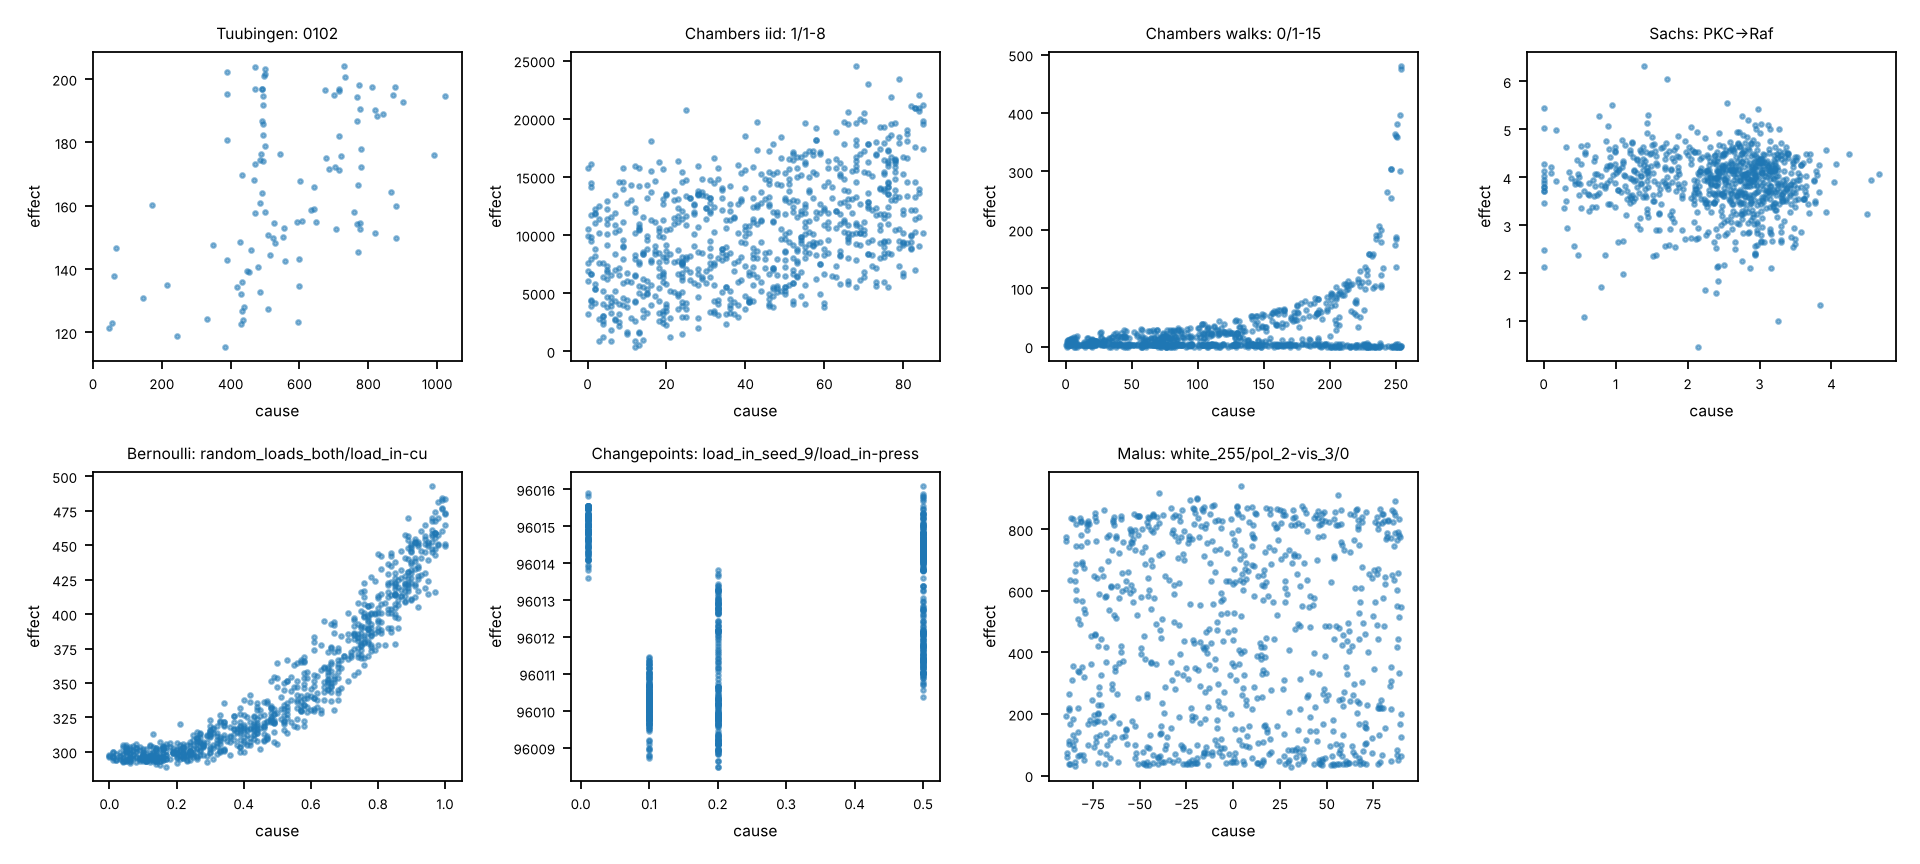
\includegraphics[width=\linewidth]{figs/examples.png}
\caption{One randomly chosen pair (seed $7$) from each collection; $800$ random rows, cause on the horizontal axis.}
\label{fig:examples}
\end{figure}



\begin{table}[t]
\caption{T\"ubingen: mean residual heteroscedasticity $h$ (true direction) on the pairs a rule orients wrongly and rightly; $p$: one-sided Mann--Whitney test that $h$ is larger on the wrong pairs. Twelve rules; $p_{\rm adj}$: Holm over the twelve.}
\label{tab:h2}
\small
\begin{tabular}{@{}lccccc@{}}
\toprule
Rule & wrong/right & $h$ wrong & $h$ right & $p$ & $p_{\rm adj}$\\
\midrule
IGCI & 45/57 & 0.19 & 0.22 & 0.707 & 1\\
RECI & 40/62 & 0.25 & 0.17 & 0.0214 & 0.165\\
ANM-HSIC & 40/62 & 0.32 & 0.13 & 2.67e-09 & 3.2e-08\\
Pairwise LiNGAM & 40/62 & 0.22 & 0.19 & 0.245 & 0.736\\
PDM & 61/41 & 0.22 & 0.18 & 0.0206 & 0.165\\
LOCI & 36/66 & 0.27 & 0.17 & 0.00141 & 0.0141\\
ANM, Gaussian process & 42/53 & 0.29 & 0.10 & 2.83e-09 & 3.2e-08\\
Compression, floor256 & 40/62 & 0.22 & 0.19 & 0.0879 & 0.452\\
Compression, floor256, raw & 36/66 & 0.22 & 0.19 & 0.0946 & 0.452\\
TRA & 29/53 & 0.26 & 0.17 & 0.00405 & 0.0365\\
Compression, round255 & 34/68 & 0.23 & 0.19 & 0.0753 & 0.452\\
AVICI & 42/60 & 0.18 & 0.22 & 0.926 & 1\\
RESIT & 37/60 & 0.34 & 0.13 & 7.98e-10 & 1.04e-08\\
\bottomrule
\end{tabular}
\end{table}

\section{Graph benchmarks}\label{sec:graphs}

The same question for graphs. We score skeletons only, against the 17-arc Sachs consensus (853 cells, log scale) and against the documented graphs of Causal Chambers recordings: two i.i.d.\ recordings (ten random subsamples of $4000$ shuffled rows each), two further recordings with an effective sample size above $1000$, and seventeen new wind-tunnel and light-tunnel recordings whose actuators are random walks and whose effective sample size, by the heuristic $n(1-\rho)/(1+\rho)$, is about three out of $4000$ rows. For the walk recordings the first $4000$ rows in time order are used. Table~\ref{tab:graphs} gives precision/recall/$F_1$ for $22$ method configurations: the classical rules (PC at two levels, GES, DirectLiNGAM, NOTEARS, DAGMA, PCMCI+), nine published packages at library defaults (experiment 45; AVICI, GOLEM, NOTEARS-MLP, GraN-DAG, DAG-GNN, GRaSP, BOSS, RESIT, CAM-UV), BF-BIC with BOSS, and the methods we developed (PC with a nonparametric test, BTAD, LRG, sequential certificates, Appendix~\ref{app:negative}).

\begin{table}[t]
\caption{Skeleton precision/recall/$F_1$ against the reference (strict), mean over data sets. Sachs: one data set; Chambers iid: $2\times10$ subsamples; ESS$>1000$: $2$ recordings; ESS$<20$: $17$ recordings. A number in parentheses is the number of data sets on which the method finished within $900$\,s when fewer than the full number. Experiments 36, 39, 43, 45.}
\label{tab:graphs}
\scriptsize
\setlength{\tabcolsep}{2pt}
\begin{tabular}{@{}lcccc@{}}
\toprule
Method & Sachs & Chambers iid & ESS $>1000$ & ESS $<20$\\
\midrule
PC $\alpha=$0.05 & 1.00/0.41/0.58 & 0.40/0.38/0.37 & 0.48/0.28/0.35 & 0.36/0.39/0.37\\
PC $\alpha=$0.01 & 1.00/0.35/0.52 & 0.39/0.33/0.34 & 0.51/0.27/0.36 & 0.36/0.36/0.36\\
GES-BIC & 1.00/0.41/0.58 & 0.45/0.64/0.49 & 0.74/0.67/0.70 & 0.26/0.71/0.38\\
DirectLiNGAM & 1.00/0.35/0.52 & 0.55/0.60/0.55 & 0.71/0.63/0.66 & 0.26/0.63/0.37\\
NOTEARS & 1.00/0.18/0.30 & 0.41/0.21/0.27 & 0.33/0.24/0.26 & 0.26/0.45/0.33\\
DAGMA & 1.00/0.29/0.45 & 0.44/0.33/0.36 & 0.44/0.41/0.39 & 0.25/0.52/0.34\\
PCMCI+ & 1.00/0.35/0.52 & 0.39/0.33/0.34 & 0.53/0.29/0.37 & 0.27/0.17/0.20\\
GRaSP & 1.00/0.35/0.52 & 0.53/0.57/0.52 & 0.78/0.63/0.68 & 0.27/0.50/0.35\\
BOSS & 1.00/0.35/0.52 & 0.57/0.61/0.55 & 0.77/0.57/0.65 & 0.29/0.54/0.37\\
BF-BIC + BOSS & 0.90/0.53/0.67 & 0.43/0.63/0.49 & 0.57/0.61/0.58 & 0.30/0.68/0.42\\
NOTEARS-MLP & 0.88/0.41/0.56 & 0.42/0.51/0.43 & 0.45/0.27/0.34 (1) & 0.17/0.25/0.21 (1)\\
GOLEM & 1.00/0.18/0.30 & 0.26/0.39/0.31 & 0.36/0.49/0.41 & 0.25/0.47/0.33\\
DAG-GNN & 1.00/0.18/0.30 & 0.36/0.45/0.36 & 0.45/0.34/0.38 & 0.27/0.45/0.34 (16)\\
GraN-DAG & 1.00/0.06/0.11 & 0.55/0.04/0.06 & 0.20/0.04/0.06 & 0.54/0.07/0.12\\
RESIT & 0.39/0.53/0.45 & 0.33/0.80/0.43 & 0.37/0.74/0.49 & 0.23/0.99/0.37\\
CAM-UV & 1.00/0.06/0.11 & 0.67/0.31/0.42 & 0.74/0.43/0.53 & 0.06/0.01/0.02 (15)\\
AVICI & 0.88/0.41/0.56 & 0.48/0.36/0.37 (14) & 0.54/0.17/0.26 & 0.36/0.23/0.28 (8)\\
PC-GCM $\alpha=$0.05 & 0.89/0.47/0.62 & 0.38/0.33/0.34 & 0.54/0.34/0.41 & 0.35/0.54/0.42\\
PC-GCM $\alpha=$0.01 & 1.00/0.47/0.64 & 0.39/0.30/0.32 & 0.47/0.26/0.33 & 0.34/0.46/0.39\\
BTAD & 0.89/0.47/0.62 & 0.56/0.36/0.41 & 0.82/0.46/0.58 & 0.60/0.16/0.25\\
LRG & 0.90/0.53/0.67 & 0.39/0.48/0.43 & 0.52/0.55/0.53 & 0.51/0.28/0.36\\
CERT-CD nonparametric & 1.00/0.29/0.45 & 0.29/0.16/0.20 & 0.60/0.18/0.28 & 0.24/0.87/0.37\\
\bottomrule
\end{tabular}
\end{table}

\paragraph{The ranking depends on the family.} On the i.i.d.\ chamber recordings the best are DirectLiNGAM and BOSS ($F_1=0.55$) and GRaSP ($0.52$); on the two recordings with a large effective sample size GES ($0.70$), GRaSP ($0.68$) and DirectLiNGAM ($0.66$); on Sachs LRG and BF-BIC with BOSS ($0.67$), PC with the nonparametric test ($0.62$--$0.64$) and BTAD ($0.62$), against $0.58$ for PC and GES. No method has a strict $F_1$ above $0.42$ on the seventeen random-walk recordings, where most methods report tens of false edges. The neural methods are weaker: GraN-DAG finds almost no edges ($F_1\le0.12$), GOLEM and DAG-GNN report $22$ to $36$ false edges per recording, NOTEARS with an MLP timed out on $16$ of $17$ walk recordings ($16$ variables) and AVICI on $9$ of $17$ and on $6$ of $20$ i.i.d.\ subsamples; their means in Table~\ref{tab:graphs} are over the data sets on which they finished and are not comparable to the others.

\paragraph{Resolution and structure of the benchmarks.} One Sachs arc changes recall by $0.06$; $16$ of $22$ configurations have a bootstrap interval that contains the best $F_1$ (Section~\ref{sec:noise}). The chamber graphs are bipartite (actuators to sensors), so skeleton recovery is feature selection from actuators to measurements, and the actuators are recognisable by their marginals (Section~\ref{sec:marg}). An interventional pilot on the light tunnel (a pilot, not pre-specified; \texttt{results/lt\_interventions\_check.json}) shows how little a graph benchmark with documented interventions leaves to a new method: a two-sample test of each sensor against the reference recording under each actuator intervention has precision $1.00$ and recall $0.72$ ($28$ of the $39$ arcs among observed variables, which here are also the ancestral pairs; AUC $0.91$ from the $p$-values), and the missed arcs, all from light sources to their sensors, show no shift in the data ($p$ between $0.06$ and $0.86$); a conditional version (residuals of a boosted regression on the estimated non-descendants) raises recall to $0.79$ at a precision of $0.51$.

\paragraph{What we do not conclude.} The reference networks are small, the Sachs consensus is contested, and several baselines (CAM, SCORE) were not run. The differences between graph methods are mostly within sampling error, and the effective sample size of the walk recordings limits what any method can show. We read the graph results as consistent with the pair results: no rule leads across families.



\section{Selective subsets}\label{app:subsets}


Pair benchmarks are often evaluated on a subset of pairs (a given variable type or sample size, or pairs where the other rules disagree). We drew $10000$ random subsets of $50$ of the $102$ pairs. The accuracy of a rule on a subset has a standard deviation of about $0.05$. For the eight rules whose full-sample accuracy is within $0.04$ of RECI the probability that a rule beats RECI on a subset lies between $0.34$ and $0.71$, so most subsets would support either order; for round255 compression, $0.059$ above RECI, it is $0.79$. The expected best accuracy over $m$ independently drawn subsets, which is what a researcher reports after trying $m$ subsets and keeping the best, grows with $m$: RECI $0.608$ ($m=1$), $0.650$ ($3$), $0.684$ ($10$); LOCI $0.647$, $0.688$, $0.722$; round255 compression $0.667$, $0.707$, $0.740$. The inflation at $m=10$ is seven to eight points for every rule, which leaves the order of the rules unchanged; what it changes is the claim of an absolute level. Each subset is half of the same $102$ pairs, so this measures selection noise about a known full-sample accuracy, not how a researcher actually chooses subsets (by type or size, not at random).







\section{Tables moved from the main text}
\begin{table}[ht]
\caption{Accuracy (fraction of pairs oriented correctly; exact ties half) of twelve rules on eight collections. All rules see the raw arrays, except that T\"ubingen is dequantised (Section~\ref{sec:rules}). ``--'': not run, or no value for most pairs (TRA on the changepoint collection; PDM and the first compression implementation only on the original collections). ``Walks (19)'' contains all $19$ untouched recordings ($486$ pairs; the $122$ pairs of ``walks'' come from five of them). The new collections have $8$, $7$ and $4$ distinct edges; intervals that account for clusters are in Appendix Table~\ref{tab:collections_ci}.}
\label{tab:collections2}
\small
\setlength{\tabcolsep}{3.2pt}
\begin{tabular}{@{}lcccccccc@{}}
\toprule
Rule & T\"ub. & iid & walks & Walks & Sachs & Bern. & Chgpt. & Malus\\
 & (102) & (94) & (122) & (19: 486) & (17) & (16) & (70) & (48)\\
\midrule
IGCI & 0.56 & 0.94 & 0.89 & 0.96 & 0.65 & 1.00 & 1.00 & 0.08\\
RECI & 0.61 & 0.98 & 0.94 & 0.83 & 0.53 & 0.25 & 1.00 & 0.56\\
ANM-HSIC & 0.61 & 0.72 & 0.63 & 0.43 & 0.59 & 0.31 & 0.57 & 0.31\\
Pairwise LiNGAM & 0.61 & 0.78 & 0.71 & 0.67 & 0.53 & 0.88 & 0.43 & 0.40\\
PDM & 0.40 & 0.93 & 0.84 & -- & -- & -- & -- & --\\
LOCI & 0.65 & 0.77 & 0.68 & -- & 0.47 & 0.56 & 0.80 & 0.38\\
ANM, Gaussian process & 0.55 & 0.77 & 0.67 & -- & 0.56 & 0.47 & 0.54 & 0.33\\
Compression, floor256 & 0.61 & 0.30 & 0.61 & -- & 0.76 & -- & -- & --\\
Compression, round255 & 0.67 & 0.38 & 0.52 & 0.50 & 0.65 & 0.50 & 1.00 & 0.60\\
TRA & 0.65 & 0.86 & 0.61 & 0.56 & 0.59 & 0.62 & -- & 0.54\\
AVICI & 0.59 & 0.90 & 0.56 & 0.63 & 0.53 & 0.62 & 0.40 & 0.02\\
RESIT & 0.61 & 0.71 & 0.65 & 0.48 & 0.47 & 0.25 & 0.53 & 0.50\\
\bottomrule
\end{tabular}
\end{table}

\begin{table}[ht]
\caption{Rules on the 102 T\"ubingen pairs: unweighted accuracy with a 95\% interval (TRA: the $82$ pairs on which it returned a value) and the multiverse summary of Section~\ref{sec:multi}. ``Range'': minimum and maximum accuracy over the ten reporting universes with at least $30$ pairs per rule; ``Rank'': best and worst rank; ``First'': universes in which the rule is first (ties share the rank); ``$>$RECI'': universes in which it is above RECI; ``Best of 10'': expected best accuracy after trying ten random subsets of $50$ pairs.}
\label{tab:multi}
\small
\setlength{\tabcolsep}{3pt}
\begin{tabular}{@{}lcccccc@{}}
\toprule
Rule & Accuracy [interval] & Range & Rank & First & $>$RECI & Best of 10\\
\midrule
IGCI & 0.559 [0.46, 0.66] & 0.47--0.71 & 4--12 & 0 & 0 & 0.635\\
RECI & 0.608 [0.51, 0.70] & 0.61--0.87 & 1--6 & 1 & 0 & 0.684\\
ANM-HSIC & 0.608 [0.51, 0.70] & 0.57--0.70 & 3--12 & 0 & 1 & 0.682\\
Pairwise LiNGAM & 0.608 [0.51, 0.70] & 0.54--0.74 & 4--13 & 0 & 0 & 0.682\\
PDM & 0.402 [0.31, 0.50] & 0.40--0.61 & 10--13 & 0 & 0 & 0.477\\
LOCI & 0.647 [0.55, 0.74] & 0.63--0.77 & 1--9 & 1 & 2 & 0.722\\
ANM, Gaussian process & 0.554 [0.45, 0.65] & 0.55--0.75 & 3--12 & 0 & 0 & 0.628\\
Compression, floor256 & 0.608 [0.51, 0.70] & 0.61--0.79 & 3--8 & 0 & 0 & 0.686\\
Compression, floor256, raw rows & 0.647 [0.55, 0.74] & 0.64--0.76 & 2--8 & 0 & 2 & 0.721\\
TRA & 0.646 [0.53, 0.75] & 0.65--0.76 & 2--6 & 0 & 4 & 0.729\\
Compression, round255 & 0.667 [0.57, 0.76] & 0.67--0.88 & 1--3 & 8 & 9 & 0.740\\
AVICI & 0.588 [0.49, 0.68] & 0.54--0.65 & 5--12 & 0 & 0 & 0.665\\
RESIT & 0.613 [0.52, 0.71] & 0.47--0.66 & 5--13 & 0 & 1 & 0.686\\
\bottomrule
\end{tabular}
\end{table}

\begin{table}[ht]
\caption{T\"ubingen, $50$ protocol configurations (five row caps $\times$ dequantisation or not $\times$ five seeds). Range of the unweighted and of the official-weight accuracy over all configurations, and the range (in points) between the best and the worst level of each factor, averaged over the others.}
\label{tab:protocol}
\small
\begin{tabular}{@{}lccccc@{}}
\toprule
Rule & unweighted & weighted & rows & dequant. & seed\\
\midrule
IGCI (ours, uniform ref.) & 0.49--0.66 & 0.57--0.68 & 1 & 11 & 1\\
RECI & 0.56--0.67 & 0.58--0.73 & 2 & 1 & 2\\
ANM-HSIC & 0.54--0.61 & 0.52--0.60 & 3 & 0 & 2\\
Pairwise LiNGAM & 0.56--0.64 & 0.58--0.67 & 2 & 0 & 3\\
Compression, round255 & 0.61--0.71 & 0.60--0.78 & 2 & 1 & 1\\
IGCI (cdt, Gaussian ref.) & 0.40--0.63 & 0.40--0.64 & 1 & 18 & 0\\
RECI (cdt) & 0.60--0.68 & 0.66--0.79 & 2 & 2 & 1\\
CDS (cdt) & 0.54--0.66 & 0.50--0.65 & 7 & 4 & 2\\
\bottomrule
\end{tabular}
\end{table}

\begin{table}[ht]
\caption{Accuracy of rules under two tie conditions (raw arrays; $10^{-6}$ range jitter on tied values), same pairs (experiment 59). T\"ubingen is dequantised in both. cdt: \texttt{cdt} package defaults.}
\label{tab:ties}
\small
\setlength{\tabcolsep}{3pt}
\begin{tabular}{@{}llccccccc@{}}
\toprule
Rule & Ties & T\"ub. & iid & walks & Sachs & Bern. & Chgpt. & Malus\\
\midrule
IGCI (ours, uniform reference) & raw & 0.56 & 0.94 & 0.89 & 0.65 & 1.00 & 1.00 & 0.08\\
IGCI (ours, uniform reference) & jitter & 0.56 & 0.06 & 0.13 & 0.47 & 0.00 & 0.00 & 0.94\\
IGCI (cdt, Gaussian reference) & raw & 0.42 & 0.94 & 0.84 & 0.47 & 1.00 & 1.00 & 0.08\\
IGCI (cdt, Gaussian reference) & jitter & 0.42 & 0.06 & 0.12 & 0.53 & 0.00 & 0.00 & 0.94\\
ANM-HSIC & raw & 0.57 & 0.73 & 0.62 & 0.59 & 0.31 & 0.57 & 0.31\\
ANM-HSIC & jitter & 0.57 & 0.72 & 0.62 & 0.59 & 0.31 & 0.47 & 0.33\\
RECI & raw & 0.61 & 0.98 & 0.94 & 0.53 & 0.25 & 1.00 & 0.56\\
RECI & jitter & 0.61 & 0.98 & 0.94 & 0.53 & 0.25 & 1.00 & 0.56\\
Pairwise LiNGAM & raw & 0.61 & 0.78 & 0.71 & 0.53 & 0.88 & 0.43 & 0.40\\
Pairwise LiNGAM & jitter & 0.61 & 0.78 & 0.71 & 0.53 & 0.88 & 0.43 & 0.40\\
\bottomrule
\end{tabular}
\end{table}

\begin{table}[ht]
\caption{Reproduction of the compression baseline on the $102$ T\"ubingen pairs (official weights). The published value is $68$ of $102$ pairs, $74.7\%$ weighted.}
\label{tab:audit}
\small
\begin{tabular}{@{}lccc@{}}
\toprule
Quantisation and rows & pairs correct & unweighted & weighted\\
\midrule
$\lfloor 256q\rfloor$, all rows & 67 & 0.657 & 0.688\\
$\lfloor 255q\rfloor$, all rows & 71 & 0.696 & 0.705\\
$\mathrm{round}(255q)$, all rows & 68 & 0.667 & 0.747\\
$\mathrm{round}(255q)$, $2000$ rows & 69 & 0.676 & 0.744\\
$\mathrm{round}(255q)$, no thinning & 69 & 0.676 & 0.753\\
$\mathrm{round}(255q)$, $500$ rows & 71 & 0.696 & 0.717\\
floor256, $2000$ random dequantised rows (experiment 42) & 62 & 0.608 & 0.680\\
\bottomrule
\end{tabular}
\end{table}

\begin{table}[ht]
\caption{T\"ubingen accuracy by tercile of $h$ ($34$ pairs per tercile; TRA $24$, $31$, $27$).}
\label{tab:strata}
\small
\begin{tabular}{@{}lccc@{}}
\toprule
Rule & low $h$ & middle & high $h$\\
\midrule
ANM-HSIC & 0.97 & 0.56 & 0.29\\
RESIT & 0.96 & 0.65 & 0.24\\
ANM, Gaussian process & 0.91 & 0.53 & 0.22\\
TRA & 0.83 & 0.68 & 0.44\\
LOCI & 0.82 & 0.62 & 0.50\\
RECI & 0.68 & 0.68 & 0.47\\
IGCI & 0.59 & 0.44 & 0.65\\
Pairwise LiNGAM & 0.65 & 0.53 & 0.65\\
Compression, round255 & 0.74 & 0.74 & 0.53\\
Compression, floor256, raw & 0.71 & 0.68 & 0.56\\
AVICI & 0.53 & 0.56 & 0.68\\
PDM & 0.56 & 0.35 & 0.29\\
\bottomrule
\end{tabular}
\end{table}

\begin{table}[ht]
\caption{Matched simulated pairs: accuracy against the strength $a$ ($100$ pairs per level). Left: noise scale depends on the cause. Right: independent random scale with the same kind of marginal (control).}
\label{tab:dose}
\small
\begin{tabular}{@{}lcccc|cccc@{}}
\toprule
 & \multicolumn{4}{c|}{scale depends on cause} & \multicolumn{4}{c}{independent scale}\\
Rule & $0$ & $0.5$ & $1$ & $1.5$ & $0$ & $0.5$ & $1$ & $1.5$\\
\midrule
ANM-HSIC & 1.00 & 0.49 & 0.12 & 0.21 & 1.00 & 1.00 & 0.99 & 0.89\\
IGCI & 0.64 & 0.72 & 0.91 & 0.99 & 0.64 & 0.73 & 0.95 & 0.99\\
RECI & 0.78 & 0.77 & 0.87 & 0.93 & 0.78 & 0.84 & 0.96 & 0.98\\
\bottomrule
\end{tabular}
\end{table}


\end{document}
